% Options for packages loaded elsewhere
\PassOptionsToPackage{unicode}{hyperref}
\PassOptionsToPackage{hyphens}{url}
%
\documentclass[
  man,floatsintext]{apa6}
\usepackage{amsmath,amssymb}
\usepackage{iftex}
\ifPDFTeX
  \usepackage[T1]{fontenc}
  \usepackage[utf8]{inputenc}
  \usepackage{textcomp} % provide euro and other symbols
\else % if luatex or xetex
  \usepackage{unicode-math} % this also loads fontspec
  \defaultfontfeatures{Scale=MatchLowercase}
  \defaultfontfeatures[\rmfamily]{Ligatures=TeX,Scale=1}
\fi
\usepackage{lmodern}
\ifPDFTeX\else
  % xetex/luatex font selection
\fi
% Use upquote if available, for straight quotes in verbatim environments
\IfFileExists{upquote.sty}{\usepackage{upquote}}{}
\IfFileExists{microtype.sty}{% use microtype if available
  \usepackage[]{microtype}
  \UseMicrotypeSet[protrusion]{basicmath} % disable protrusion for tt fonts
}{}
\makeatletter
\@ifundefined{KOMAClassName}{% if non-KOMA class
  \IfFileExists{parskip.sty}{%
    \usepackage{parskip}
  }{% else
    \setlength{\parindent}{0pt}
    \setlength{\parskip}{6pt plus 2pt minus 1pt}}
}{% if KOMA class
  \KOMAoptions{parskip=half}}
\makeatother
\usepackage{xcolor}
\usepackage{longtable,booktabs,array}
\usepackage{calc} % for calculating minipage widths
% Correct order of tables after \paragraph or \subparagraph
\usepackage{etoolbox}
\makeatletter
\patchcmd\longtable{\par}{\if@noskipsec\mbox{}\fi\par}{}{}
\makeatother
% Allow footnotes in longtable head/foot
\IfFileExists{footnotehyper.sty}{\usepackage{footnotehyper}}{\usepackage{footnote}}
\makesavenoteenv{longtable}
\usepackage{graphicx}
\makeatletter
\newsavebox\pandoc@box
\newcommand*\pandocbounded[1]{% scales image to fit in text height/width
  \sbox\pandoc@box{#1}%
  \Gscale@div\@tempa{\textheight}{\dimexpr\ht\pandoc@box+\dp\pandoc@box\relax}%
  \Gscale@div\@tempb{\linewidth}{\wd\pandoc@box}%
  \ifdim\@tempb\p@<\@tempa\p@\let\@tempa\@tempb\fi% select the smaller of both
  \ifdim\@tempa\p@<\p@\scalebox{\@tempa}{\usebox\pandoc@box}%
  \else\usebox{\pandoc@box}%
  \fi%
}
% Set default figure placement to htbp
\def\fps@figure{htbp}
\makeatother
\setlength{\emergencystretch}{3em} % prevent overfull lines
\providecommand{\tightlist}{%
  \setlength{\itemsep}{0pt}\setlength{\parskip}{0pt}}
\setcounter{secnumdepth}{-\maxdimen} % remove section numbering
% Make \paragraph and \subparagraph free-standing
\makeatletter
\ifx\paragraph\undefined\else
  \let\oldparagraph\paragraph
  \renewcommand{\paragraph}{
    \@ifstar
      \xxxParagraphStar
      \xxxParagraphNoStar
  }
  \newcommand{\xxxParagraphStar}[1]{\oldparagraph*{#1}\mbox{}}
  \newcommand{\xxxParagraphNoStar}[1]{\oldparagraph{#1}\mbox{}}
\fi
\ifx\subparagraph\undefined\else
  \let\oldsubparagraph\subparagraph
  \renewcommand{\subparagraph}{
    \@ifstar
      \xxxSubParagraphStar
      \xxxSubParagraphNoStar
  }
  \newcommand{\xxxSubParagraphStar}[1]{\oldsubparagraph*{#1}\mbox{}}
  \newcommand{\xxxSubParagraphNoStar}[1]{\oldsubparagraph{#1}\mbox{}}
\fi
\makeatother
% definitions for citeproc citations
\NewDocumentCommand\citeproctext{}{}
\NewDocumentCommand\citeproc{mm}{%
  \begingroup\def\citeproctext{#2}\cite{#1}\endgroup}
\makeatletter
 % allow citations to break across lines
 \let\@cite@ofmt\@firstofone
 % avoid brackets around text for \cite:
 \def\@biblabel#1{}
 \def\@cite#1#2{{#1\if@tempswa , #2\fi}}
\makeatother
\newlength{\cslhangindent}
\setlength{\cslhangindent}{1.5em}
\newlength{\csllabelwidth}
\setlength{\csllabelwidth}{3em}
\newenvironment{CSLReferences}[2] % #1 hanging-indent, #2 entry-spacing
 {\begin{list}{}{%
  \setlength{\itemindent}{0pt}
  \setlength{\leftmargin}{0pt}
  \setlength{\parsep}{0pt}
  % turn on hanging indent if param 1 is 1
  \ifodd #1
   \setlength{\leftmargin}{\cslhangindent}
   \setlength{\itemindent}{-1\cslhangindent}
  \fi
  % set entry spacing
  \setlength{\itemsep}{#2\baselineskip}}}
 {\end{list}}
\usepackage{calc}
\newcommand{\CSLBlock}[1]{\hfill\break\parbox[t]{\linewidth}{\strut\ignorespaces#1\strut}}
\newcommand{\CSLLeftMargin}[1]{\parbox[t]{\csllabelwidth}{\strut#1\strut}}
\newcommand{\CSLRightInline}[1]{\parbox[t]{\linewidth - \csllabelwidth}{\strut#1\strut}}
\newcommand{\CSLIndent}[1]{\hspace{\cslhangindent}#1}
\ifLuaTeX
\usepackage[bidi=basic]{babel}
\else
\usepackage[bidi=default]{babel}
\fi
\babelprovide[main,import]{english}
% get rid of language-specific shorthands (see #6817):
\let\LanguageShortHands\languageshorthands
\def\languageshorthands#1{}
\ifLuaTeX
  \usepackage[english]{selnolig} % disable illegal ligatures
\fi
% Manuscript styling
\usepackage{upgreek}
\captionsetup{font=singlespacing,justification=justified}

% Table formatting
\usepackage{longtable}
\usepackage{lscape}
% \usepackage[counterclockwise]{rotating}   % Landscape page setup for large tables
\usepackage{multirow}		% Table styling
\usepackage{tabularx}		% Control Column width
\usepackage[flushleft]{threeparttable}	% Allows for three part tables with a specified notes section
\usepackage{threeparttablex}            % Lets threeparttable work with longtable

% Create new environments so endfloat can handle them
% \newenvironment{ltable}
%   {\begin{landscape}\centering\begin{threeparttable}}
%   {\end{threeparttable}\end{landscape}}
\newenvironment{lltable}{\begin{landscape}\centering\begin{ThreePartTable}}{\end{ThreePartTable}\end{landscape}}

% Enables adjusting longtable caption width to table width
% Solution found at http://golatex.de/longtable-mit-caption-so-breit-wie-die-tabelle-t15767.html
\makeatletter
\newcommand\LastLTentrywidth{1em}
\newlength\longtablewidth
\setlength{\longtablewidth}{1in}
\newcommand{\getlongtablewidth}{\begingroup \ifcsname LT@\roman{LT@tables}\endcsname \global\longtablewidth=0pt \renewcommand{\LT@entry}[2]{\global\advance\longtablewidth by ##2\relax\gdef\LastLTentrywidth{##2}}\@nameuse{LT@\roman{LT@tables}} \fi \endgroup}

% \setlength{\parindent}{0.5in}
% \setlength{\parskip}{0pt plus 0pt minus 0pt}

% Overwrite redefinition of paragraph and subparagraph by the default LaTeX template
% See https://github.com/crsh/papaja/issues/292
\makeatletter
\renewcommand{\paragraph}{\@startsection{paragraph}{4}{\parindent}%
  {0\baselineskip \@plus 0.2ex \@minus 0.2ex}%
  {-1em}%
  {\normalfont\normalsize\bfseries\itshape\typesectitle}}

\renewcommand{\subparagraph}[1]{\@startsection{subparagraph}{5}{1em}%
  {0\baselineskip \@plus 0.2ex \@minus 0.2ex}%
  {-\z@\relax}%
  {\normalfont\normalsize\itshape\hspace{\parindent}{#1}\textit{\addperi}}{\relax}}
\makeatother

\makeatletter
\usepackage{etoolbox}
\patchcmd{\maketitle}
  {\section{\normalfont\normalsize\abstractname}}
  {\section*{\normalfont\normalsize\abstractname}}
  {}{\typeout{Failed to patch abstract.}}
\patchcmd{\maketitle}
  {\section{\protect\normalfont{\@title}}}
  {\section*{\protect\normalfont{\@title}}}
  {}{\typeout{Failed to patch title.}}
\makeatother

\usepackage{xpatch}
\makeatletter
\xapptocmd\appendix
  {\xapptocmd\section
    {\addcontentsline{toc}{section}{\appendixname\ifoneappendix\else~\theappendix\fi: #1}}
    {}{\InnerPatchFailed}%
  }
{}{\PatchFailed}
\makeatother
\usepackage{csquotes}
\usepackage{bookmark}
\IfFileExists{xurl.sty}{\usepackage{xurl}}{} % add URL line breaks if available
\urlstyle{same}
\hypersetup{
  pdftitle={Data Science Exam},
  pdfauthor={Precious Nhamo},
  pdflang={en-EN},
  hidelinks,
  pdfcreator={LaTeX via pandoc}}

\title{Data Science Exam}
\author{Precious Nhamo\textsuperscript{}}
\date{}


\shorttitle{SHORT TITLE}

\affiliation{\phantom{0}}

\abstract{%
This document comprises the responses to \textbf{Questions 1 to 5} of the 2025 Data Science examination,
along with separate analyses (e.g., a PowerPoint presentation) completed in accordance with the exam
instructions and organised within the designated folder.
}



\begin{document}
\maketitle

\section{Question1 Baby Names}\label{question1-baby-names}

We report how we determined our sample size, all data exclusions (if any), all manipulations, and all measures in the study.

\section{Question2 Music Taste}\label{question2-music-taste}

\begin{figure}

{\centering 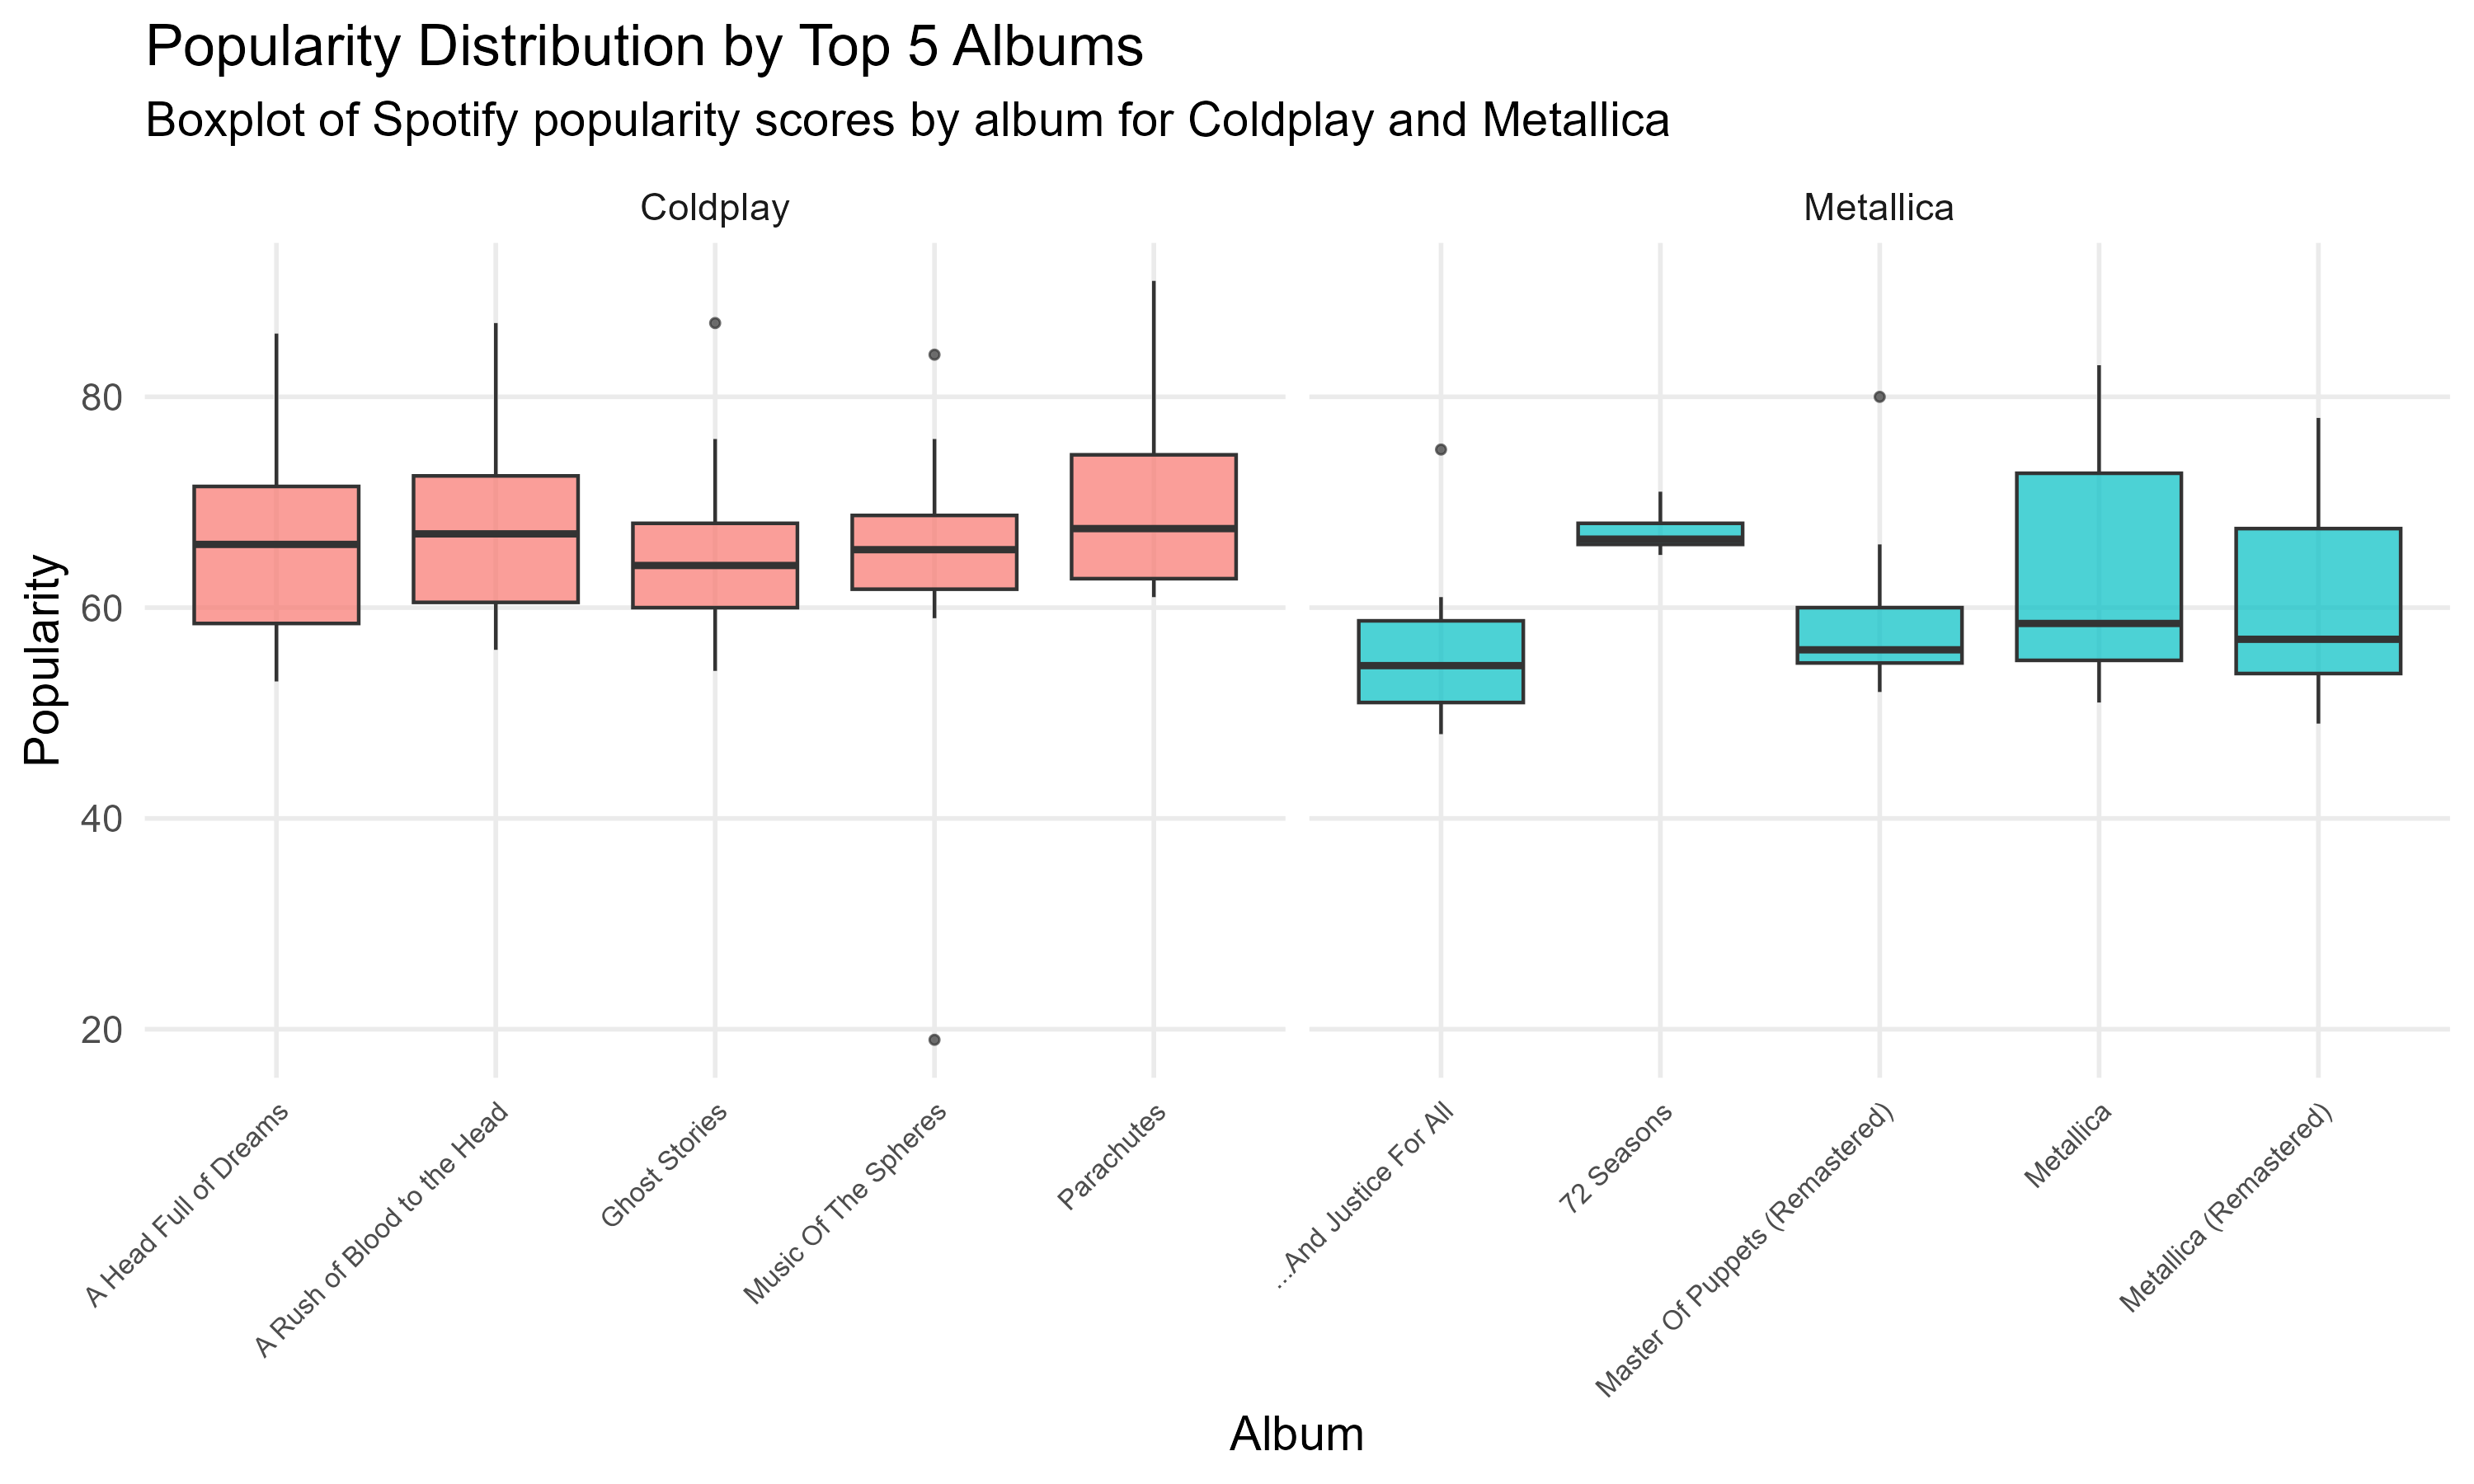
\includegraphics[width=0.9\linewidth]{../Question2/Results/popalbums} 

}

\caption{ }\label{fig:include-image-1}
\end{figure}
\begin{figure}

{\centering 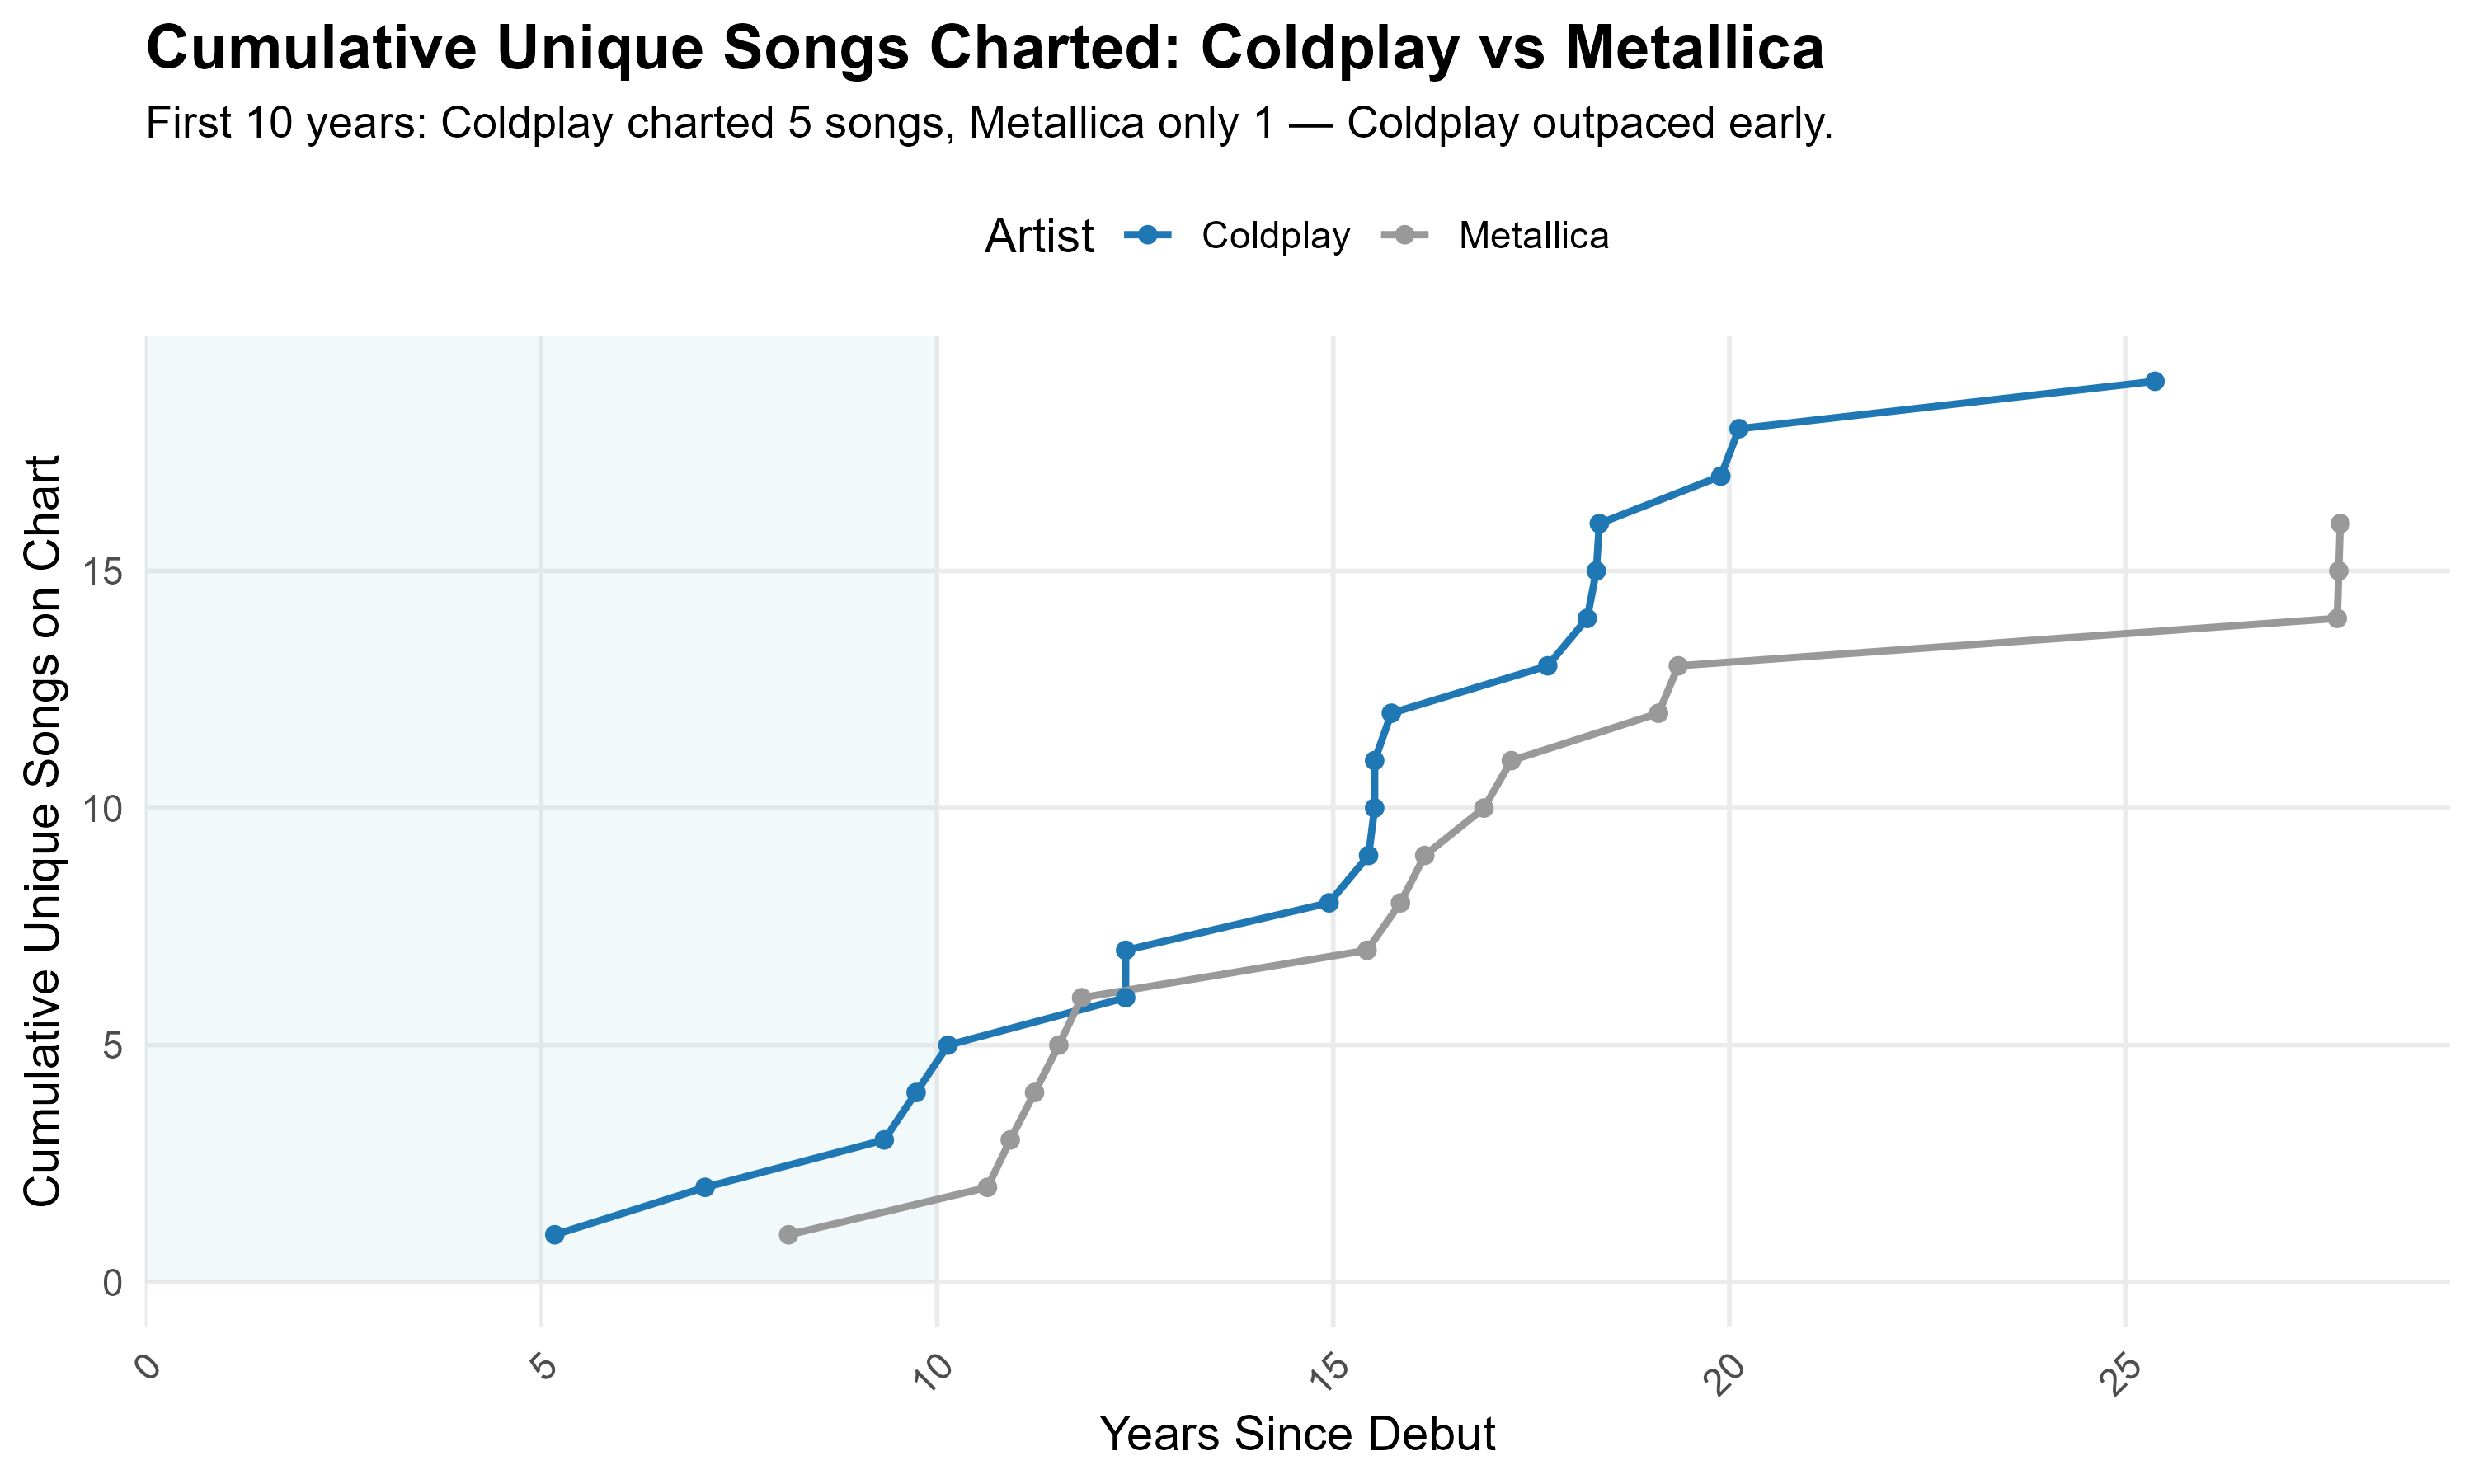
\includegraphics[width=0.9\linewidth]{../Question2/Results/uniquesongs} 

}

\caption{ }\label{fig:include-image-2}
\end{figure}
\begin{figure}

{\centering 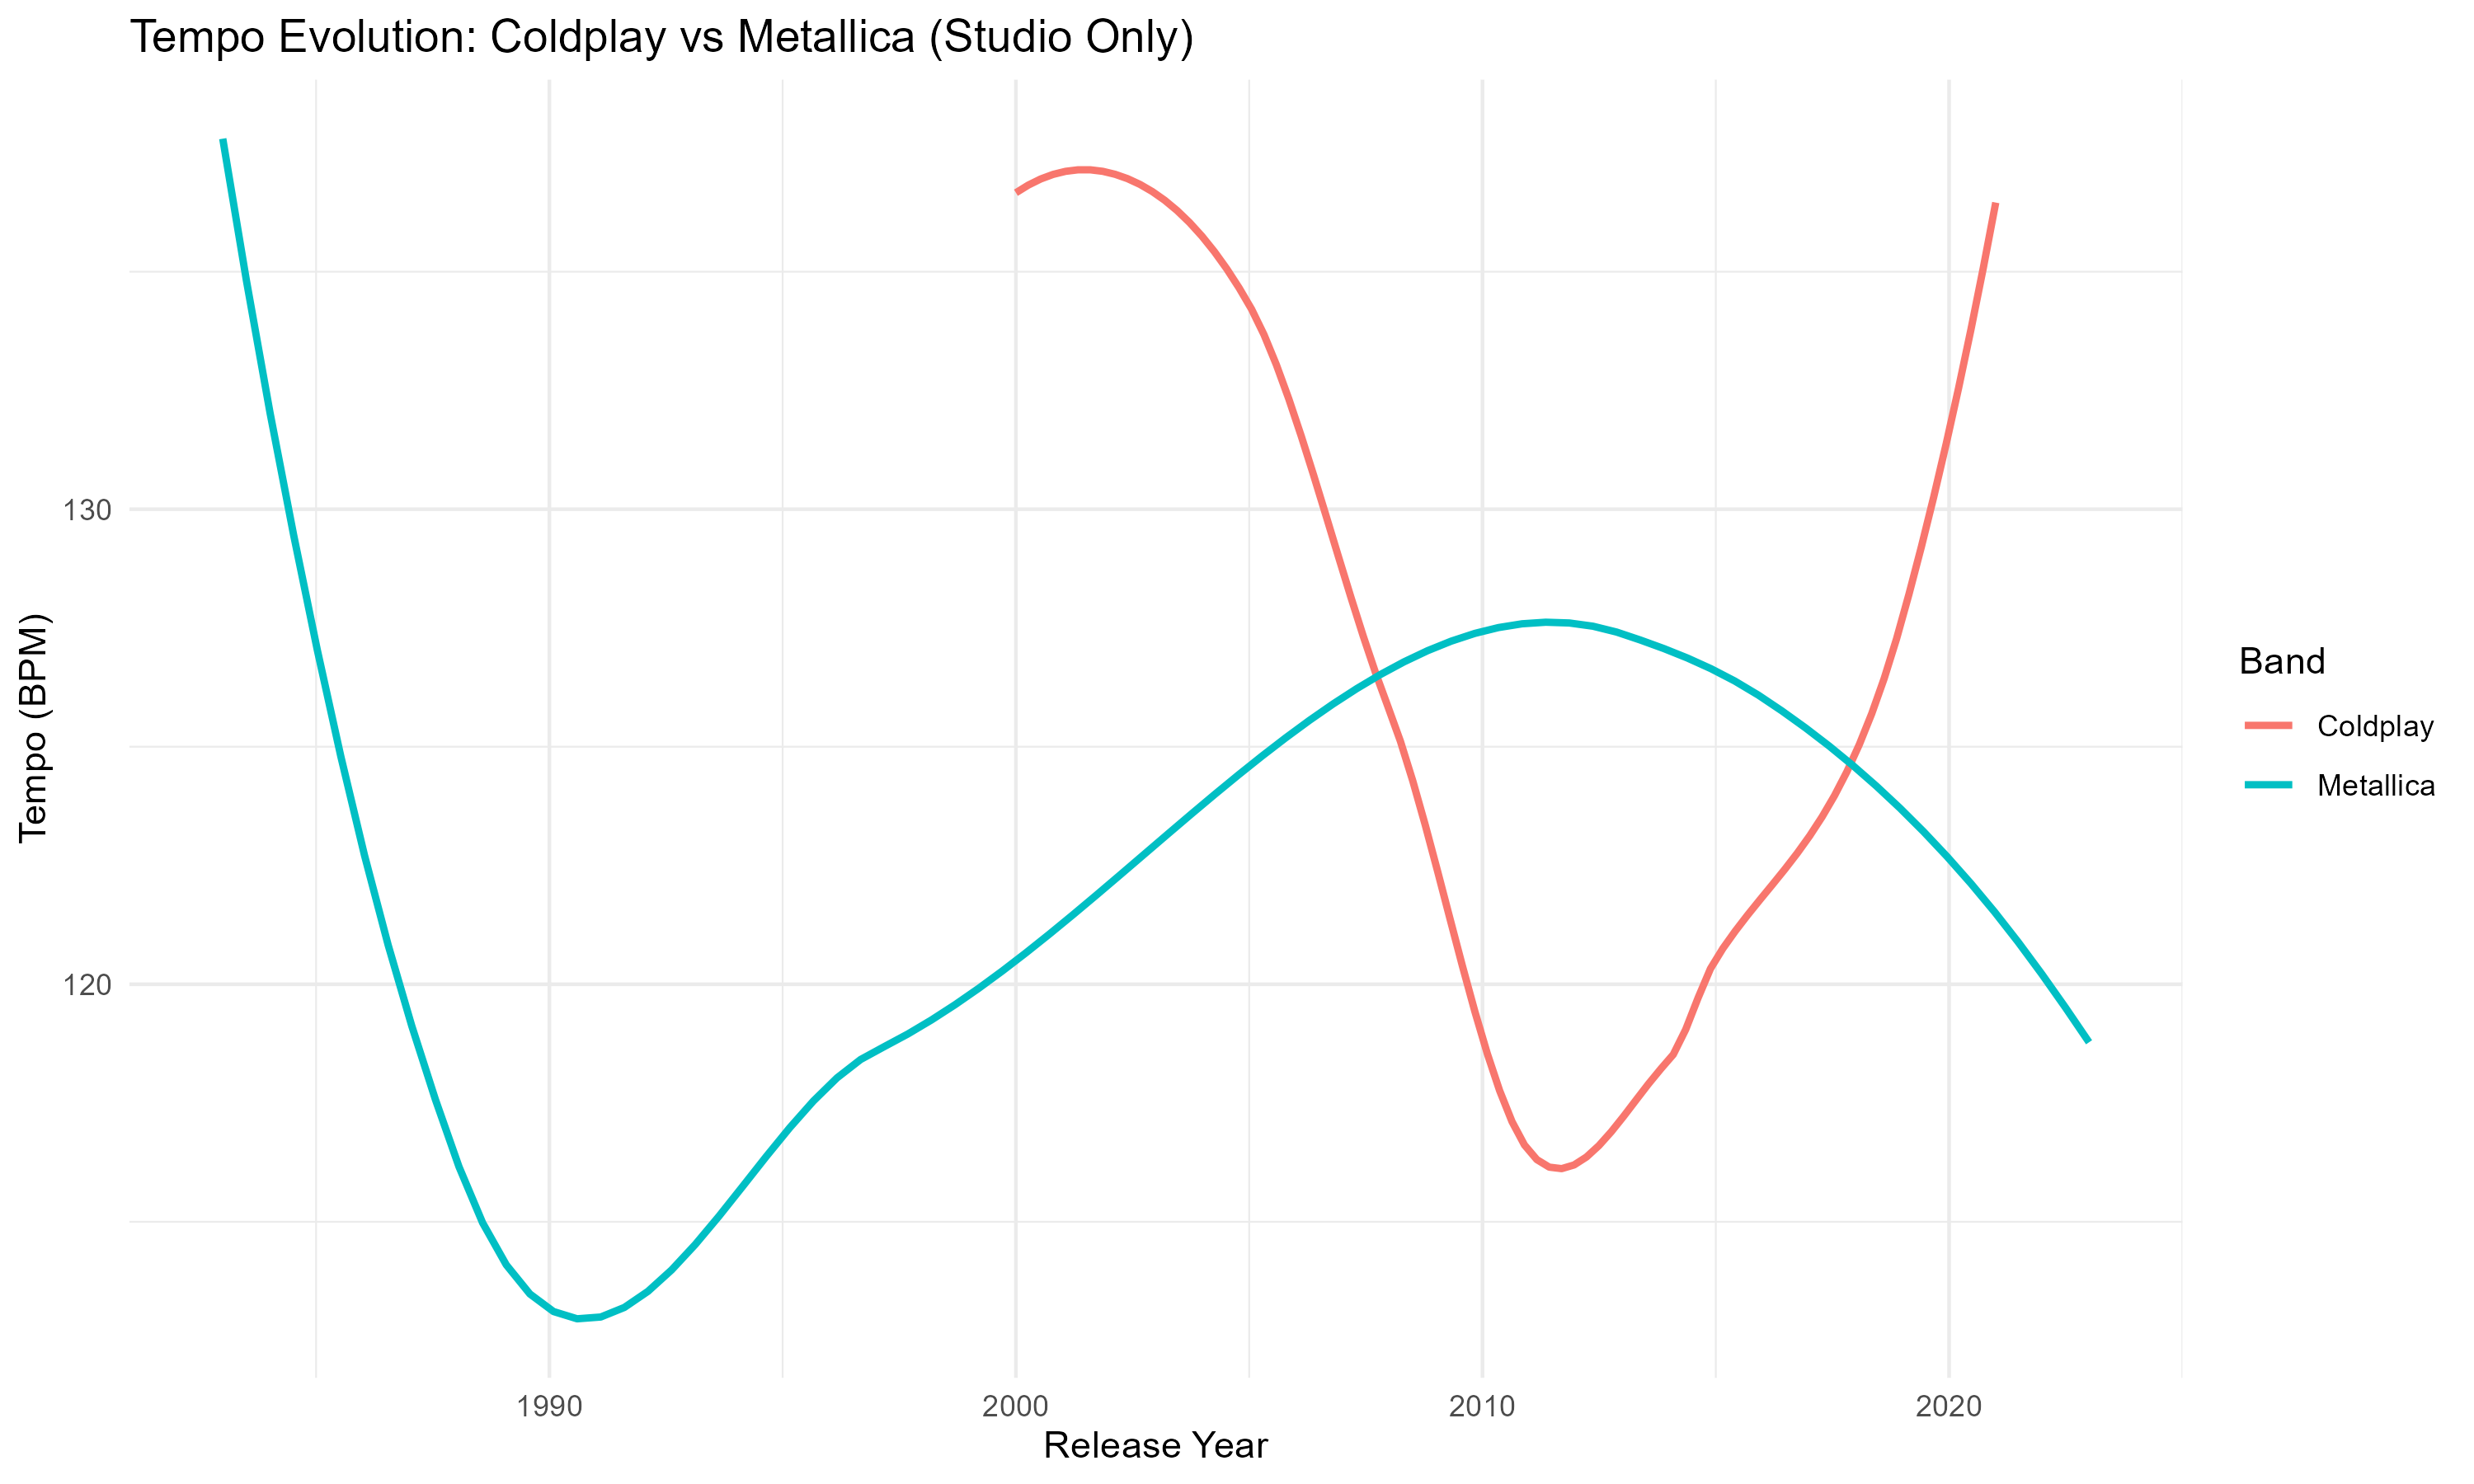
\includegraphics[width=0.9\linewidth]{../Question2/Results/audioeffects} 

}

\caption{ }\label{fig:include-image-3}
\end{figure}
\begin{figure}

{\centering 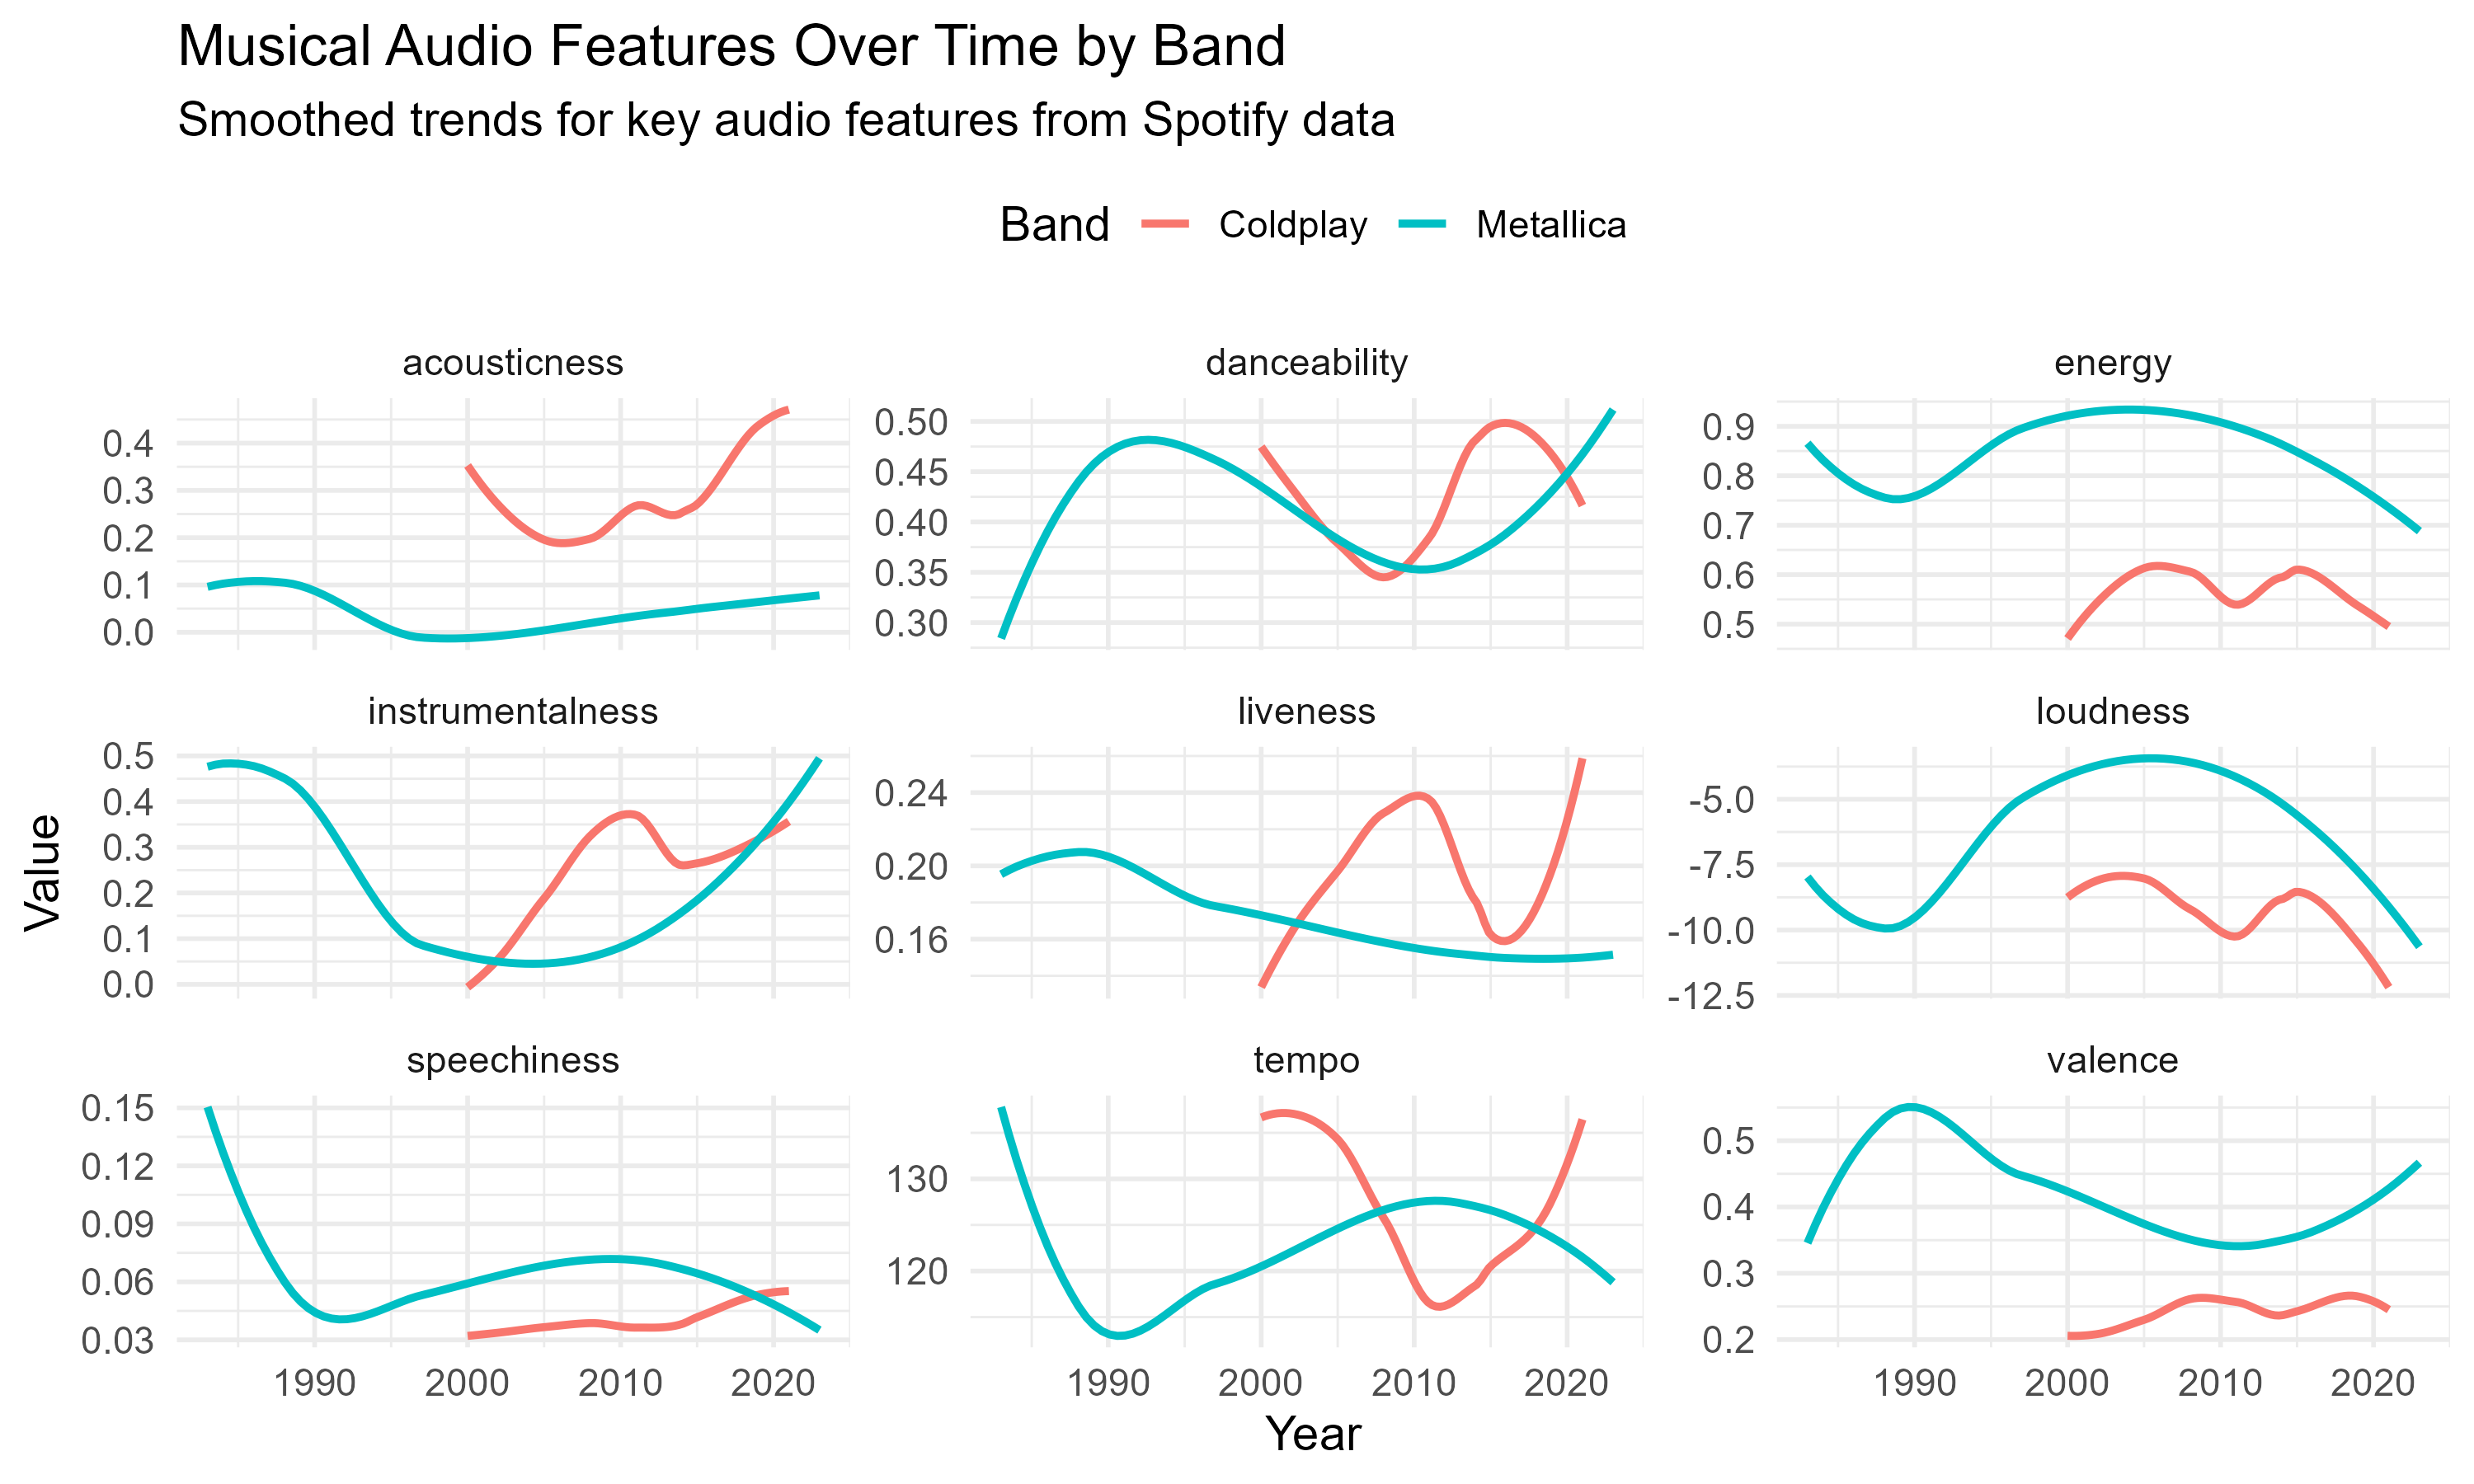
\includegraphics[width=0.9\linewidth]{../Question2/Results/extraeffects} 

}

\caption{ }\label{fig:include-image-4}
\end{figure}
\begin{figure}

{\centering 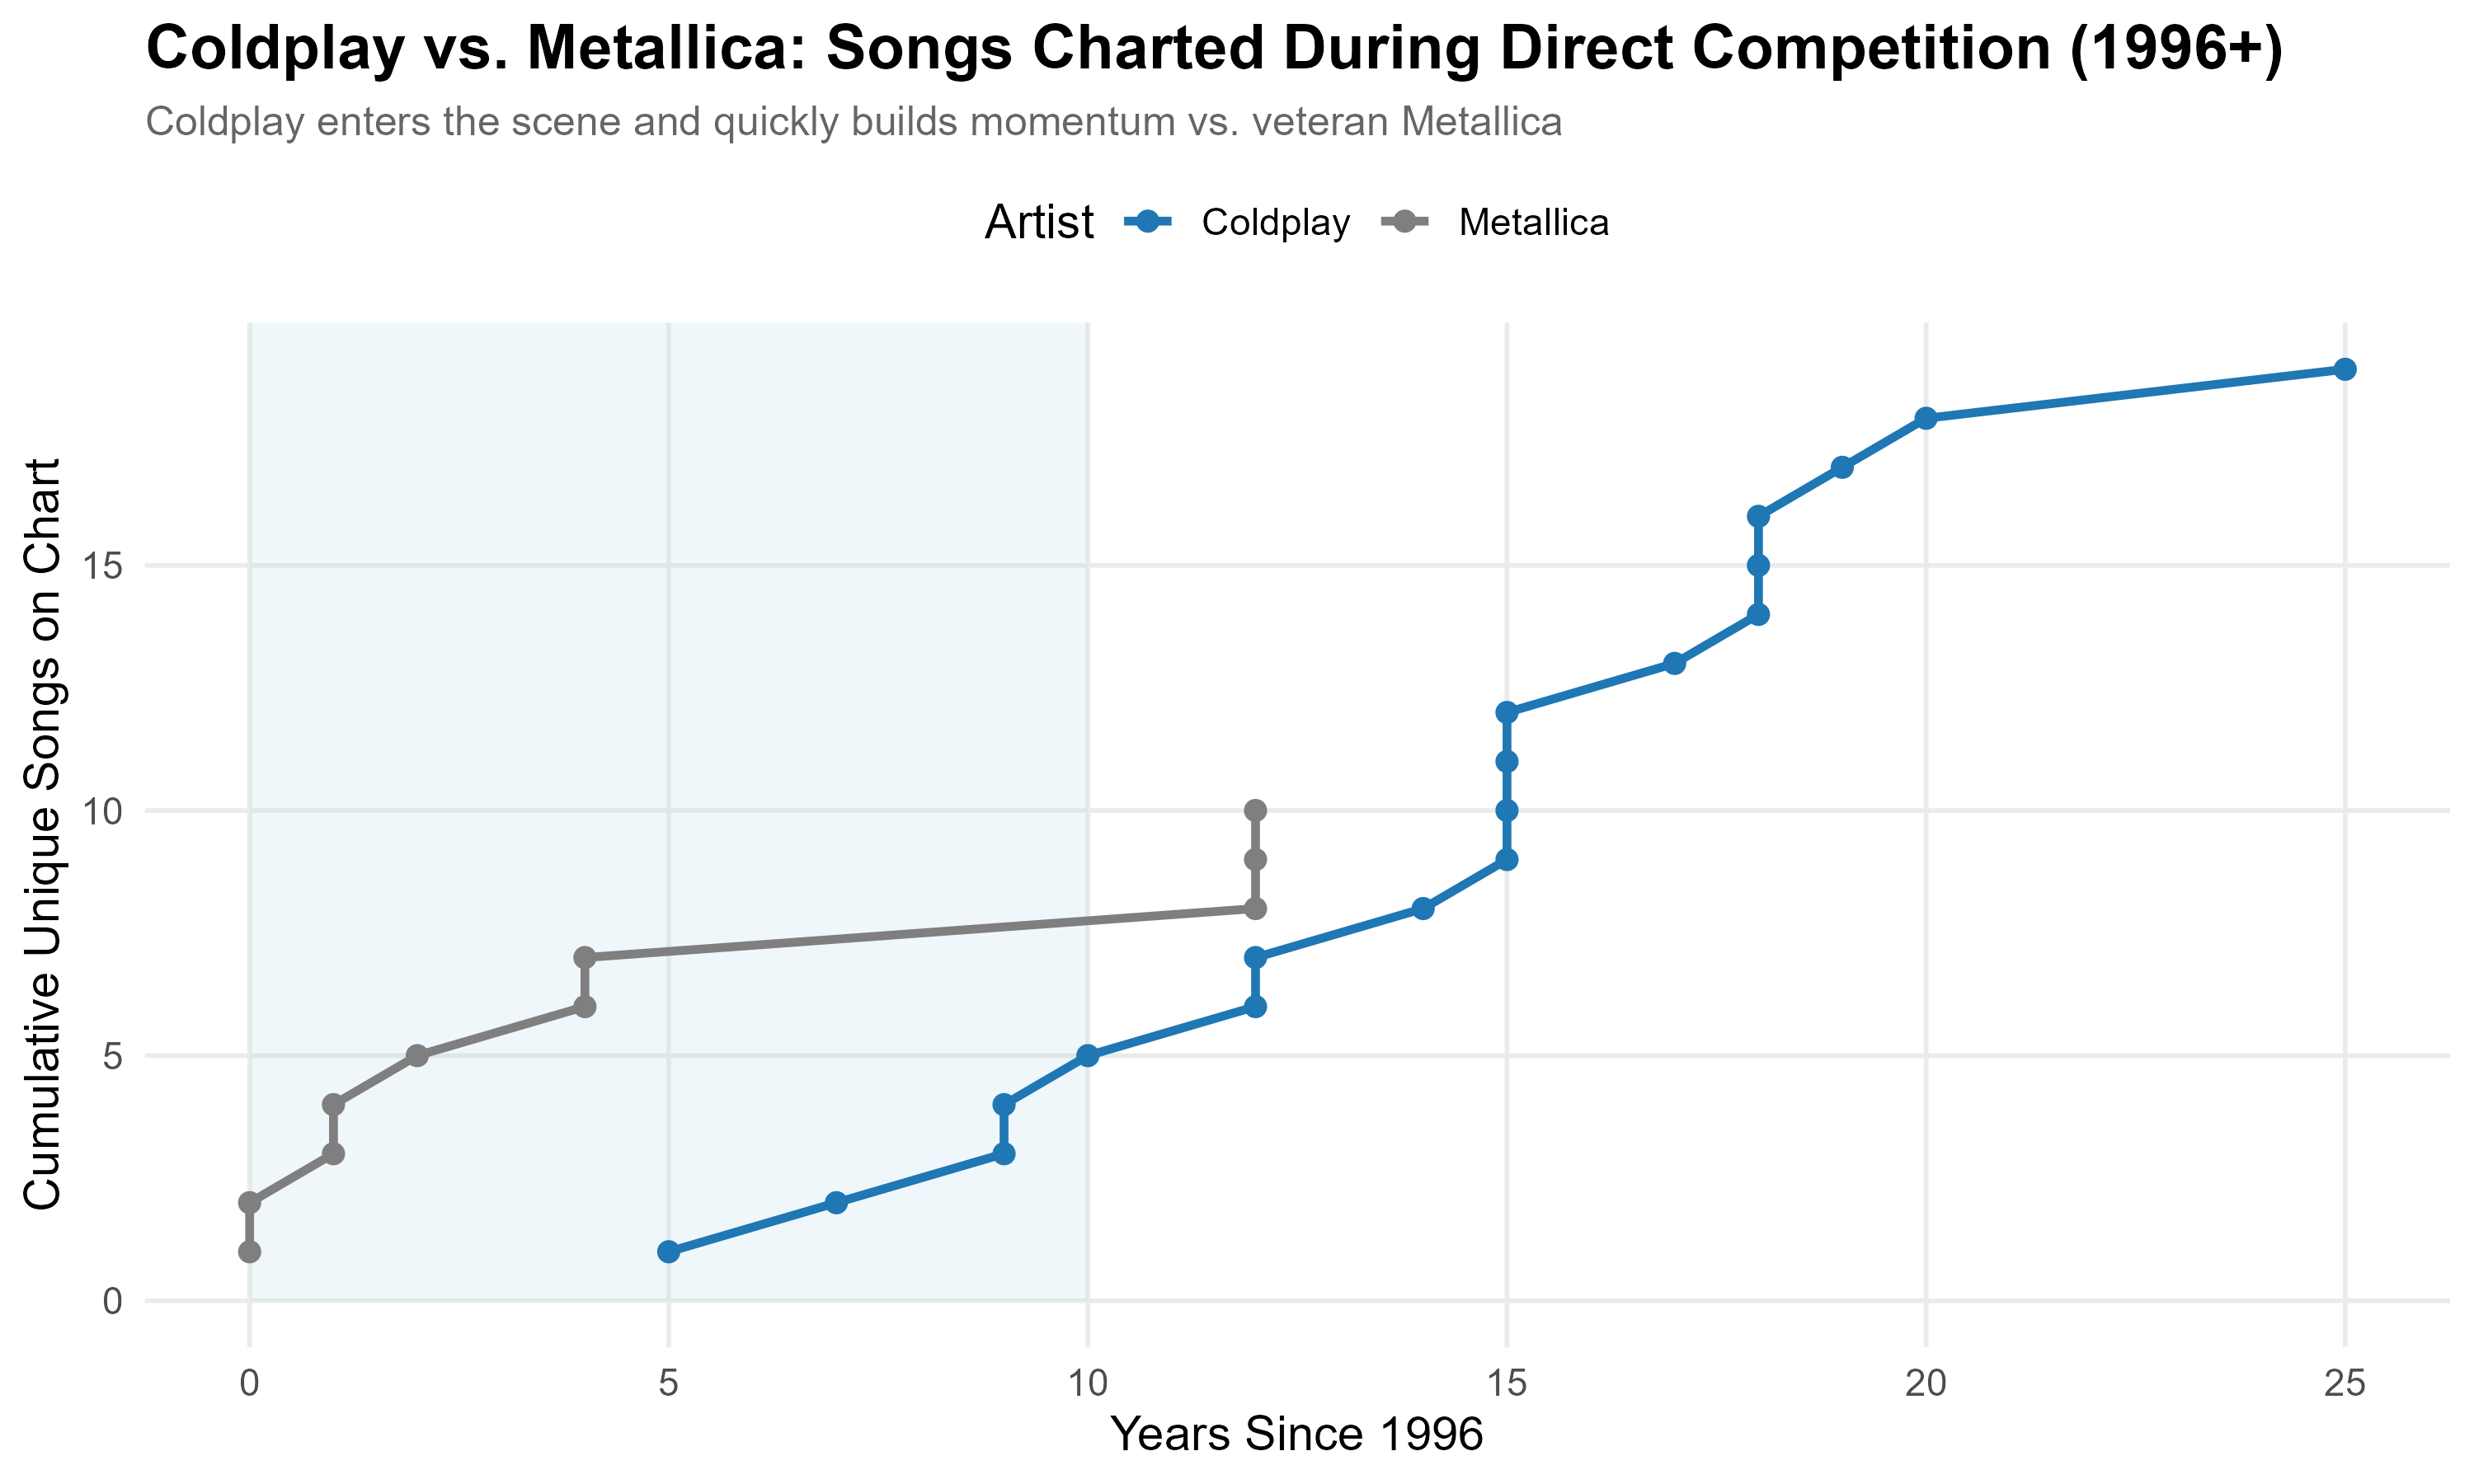
\includegraphics[width=0.9\linewidth]{../Question2/Results/directcompetition} 

}

\caption{ }\label{fig:include-image-5}
\end{figure}
\begin{figure}

{\centering 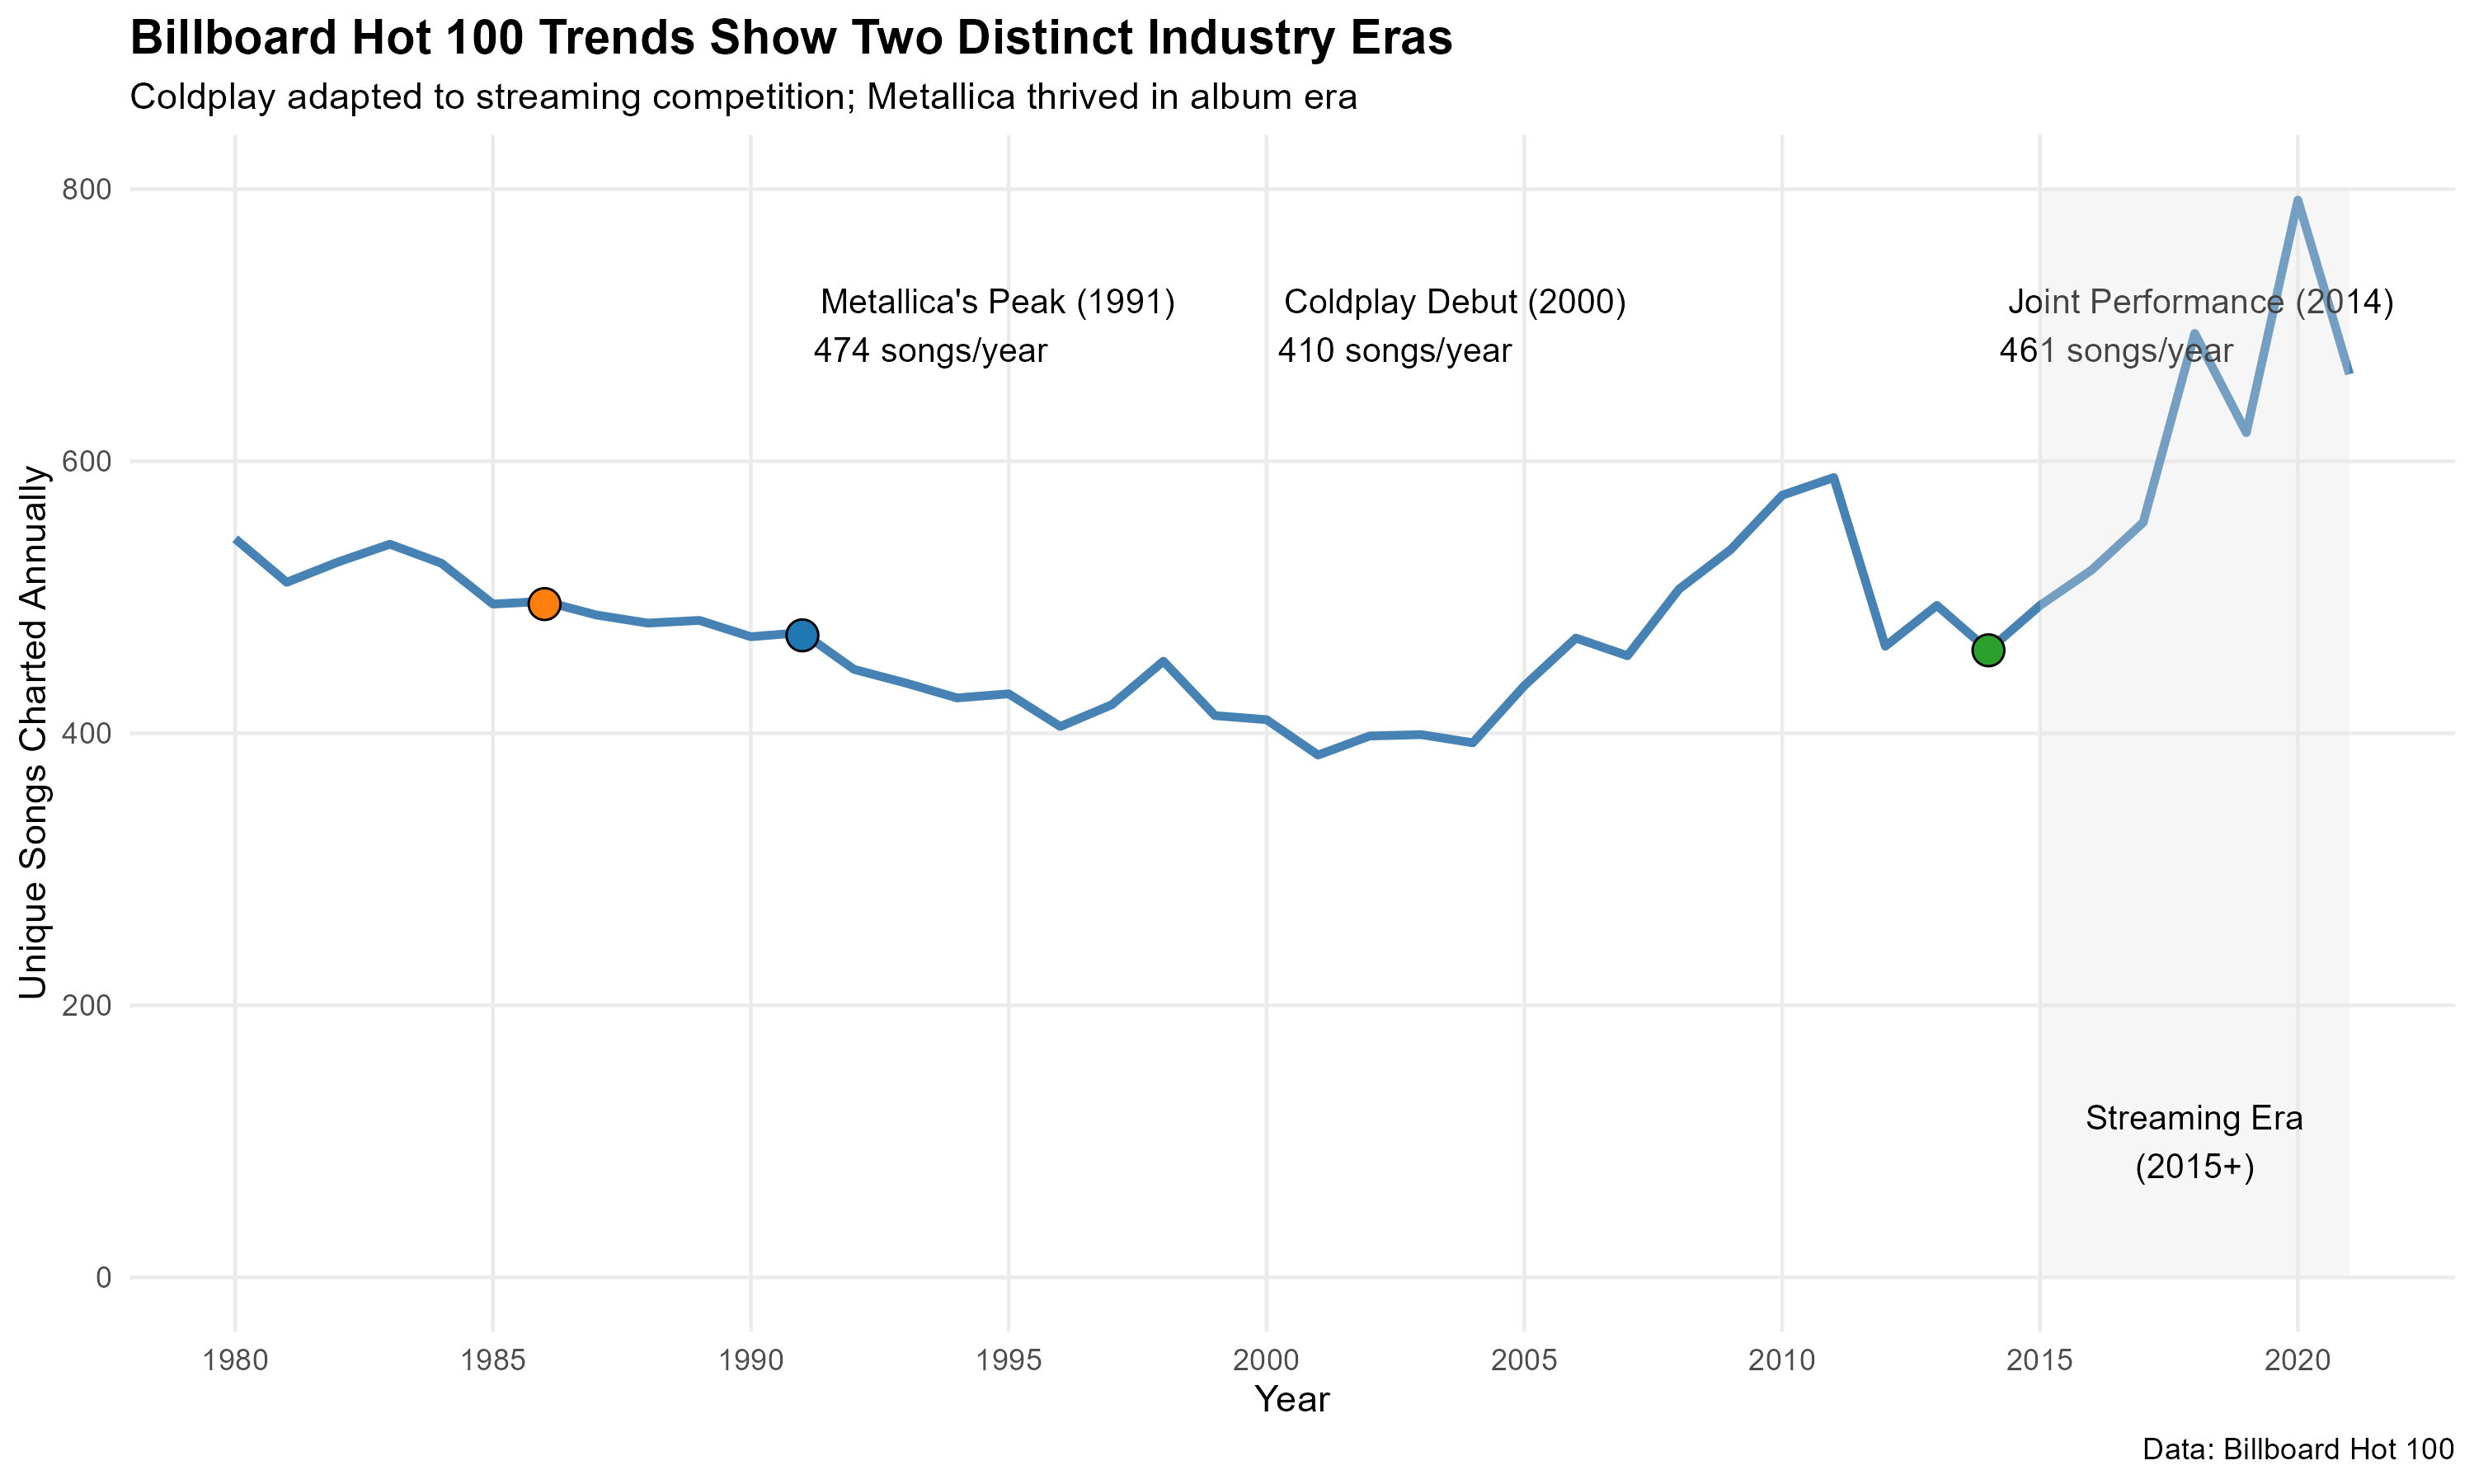
\includegraphics[width=0.9\linewidth]{../Question2/Results/industrytrend} 

}

\caption{ }\label{fig:include-image-6}
\end{figure}

\subsection{Longevity and Musical Progression of Coldplay and Metallica}\label{longevity-and-musical-progression-of-coldplay-and-metallica}

The data reveals distinct trajectories for Coldplay and Metallica in terms of popularity, musical evolution, and industry adaptation. Coldplay demonstrated early dominance, charting five songs in their first decade compared to Metallica's one (Figure 2). Their popularity scores on Spotify also show broader appeal, with a higher median and narrower interquartile range than Metallica's (Figure 1).

Musically, Coldplay's tempo has remained stable (Figure 3), while their audio features, such as danceability and valence, trended positively over time (Figure 4). Metallica, conversely, maintained higher instrumentalness and energy, reflecting their heavier style.

Billboard data highlights their adaptation to industry shifts: Metallica peaked during the album era (1991), while Coldplay thrived post-2000, leveraging streaming's rise (Figure 6). During direct competition (1996+), Coldplay's momentum outpaced Metallica's (Figure 5).

Coldplay's consistent, accessible sound contrasts with Metallica's enduring heavy metal identity. Both bands exemplify longevity but reflect divergent strategies in navigating musical trends

\section{Question 3 : Netflix Content Strategy Analysis}\label{question-3-netflix-content-strategy-analysis}

In light of Netflix's recent subscriber attrition and share price volatility, a strategic review was conducted to inform potential market entry for a new streaming venture. This review draws on IMDb ratings and global production data to assess what drives success in streaming content.

\begin{figure}

{\centering 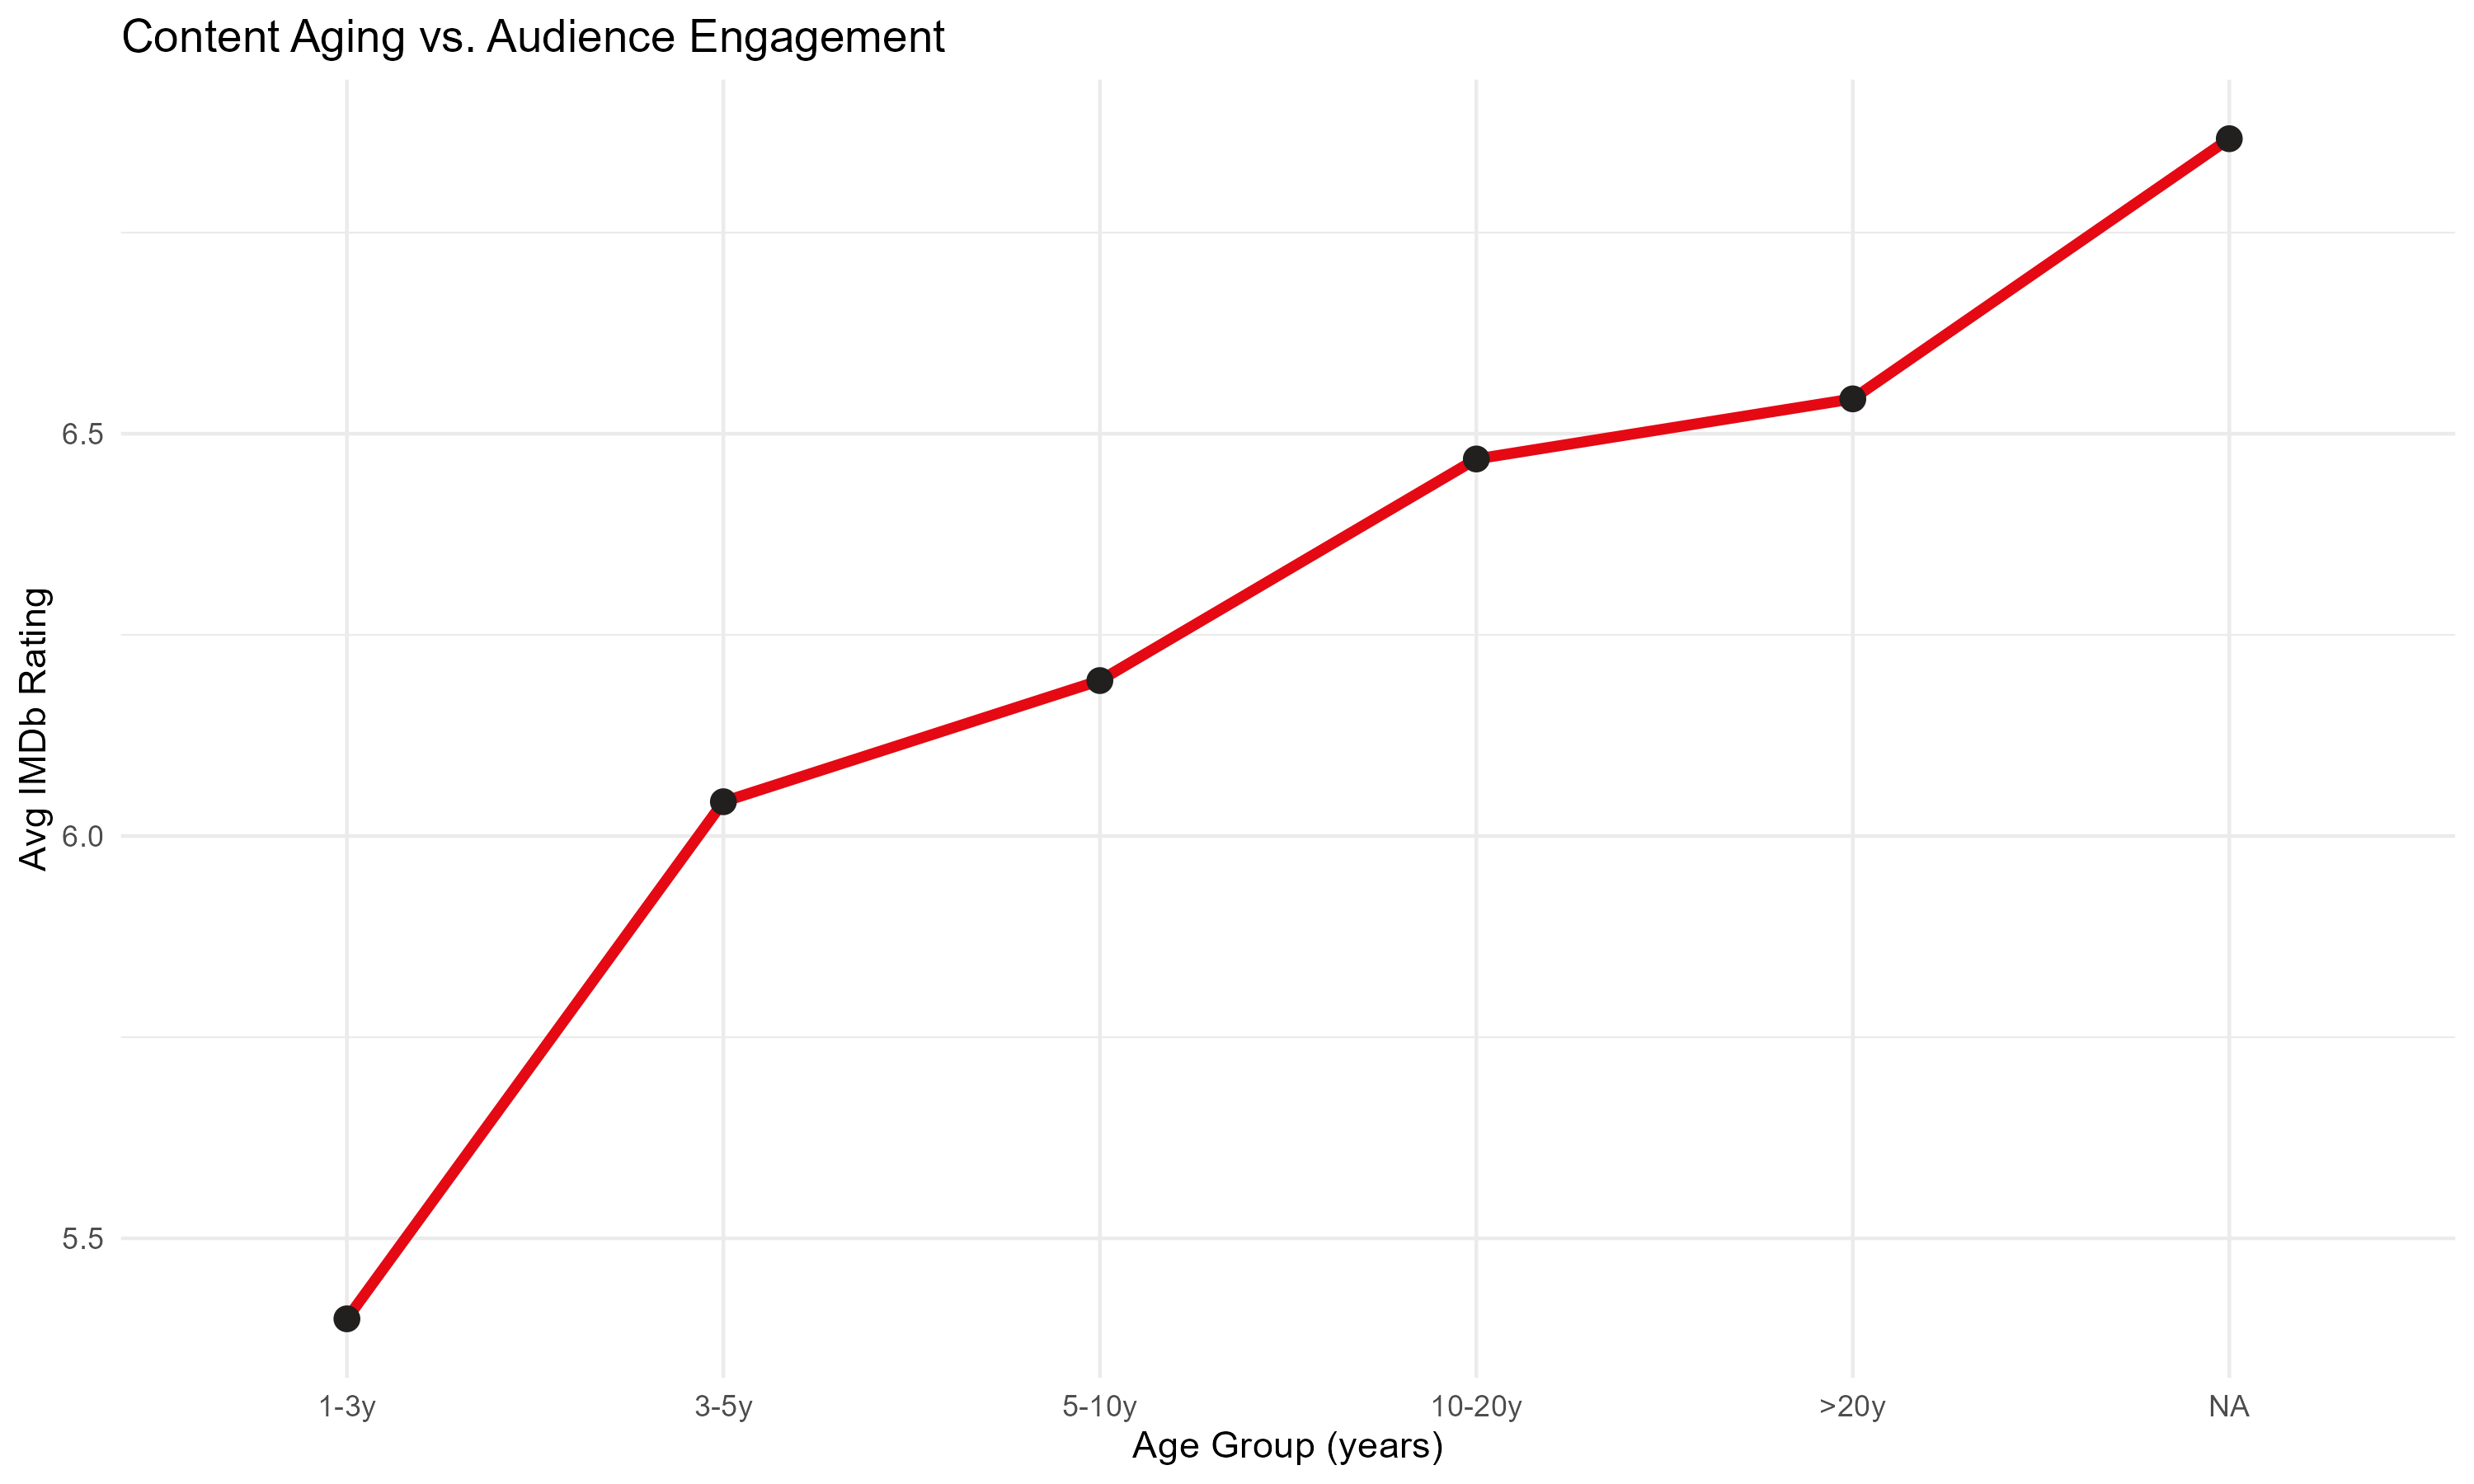
\includegraphics[width=0.9\linewidth]{../Question3/Results/audienceengage} 

}

\caption{ }\label{fig:audienceengage-1}
\end{figure}
\begin{figure}

{\centering 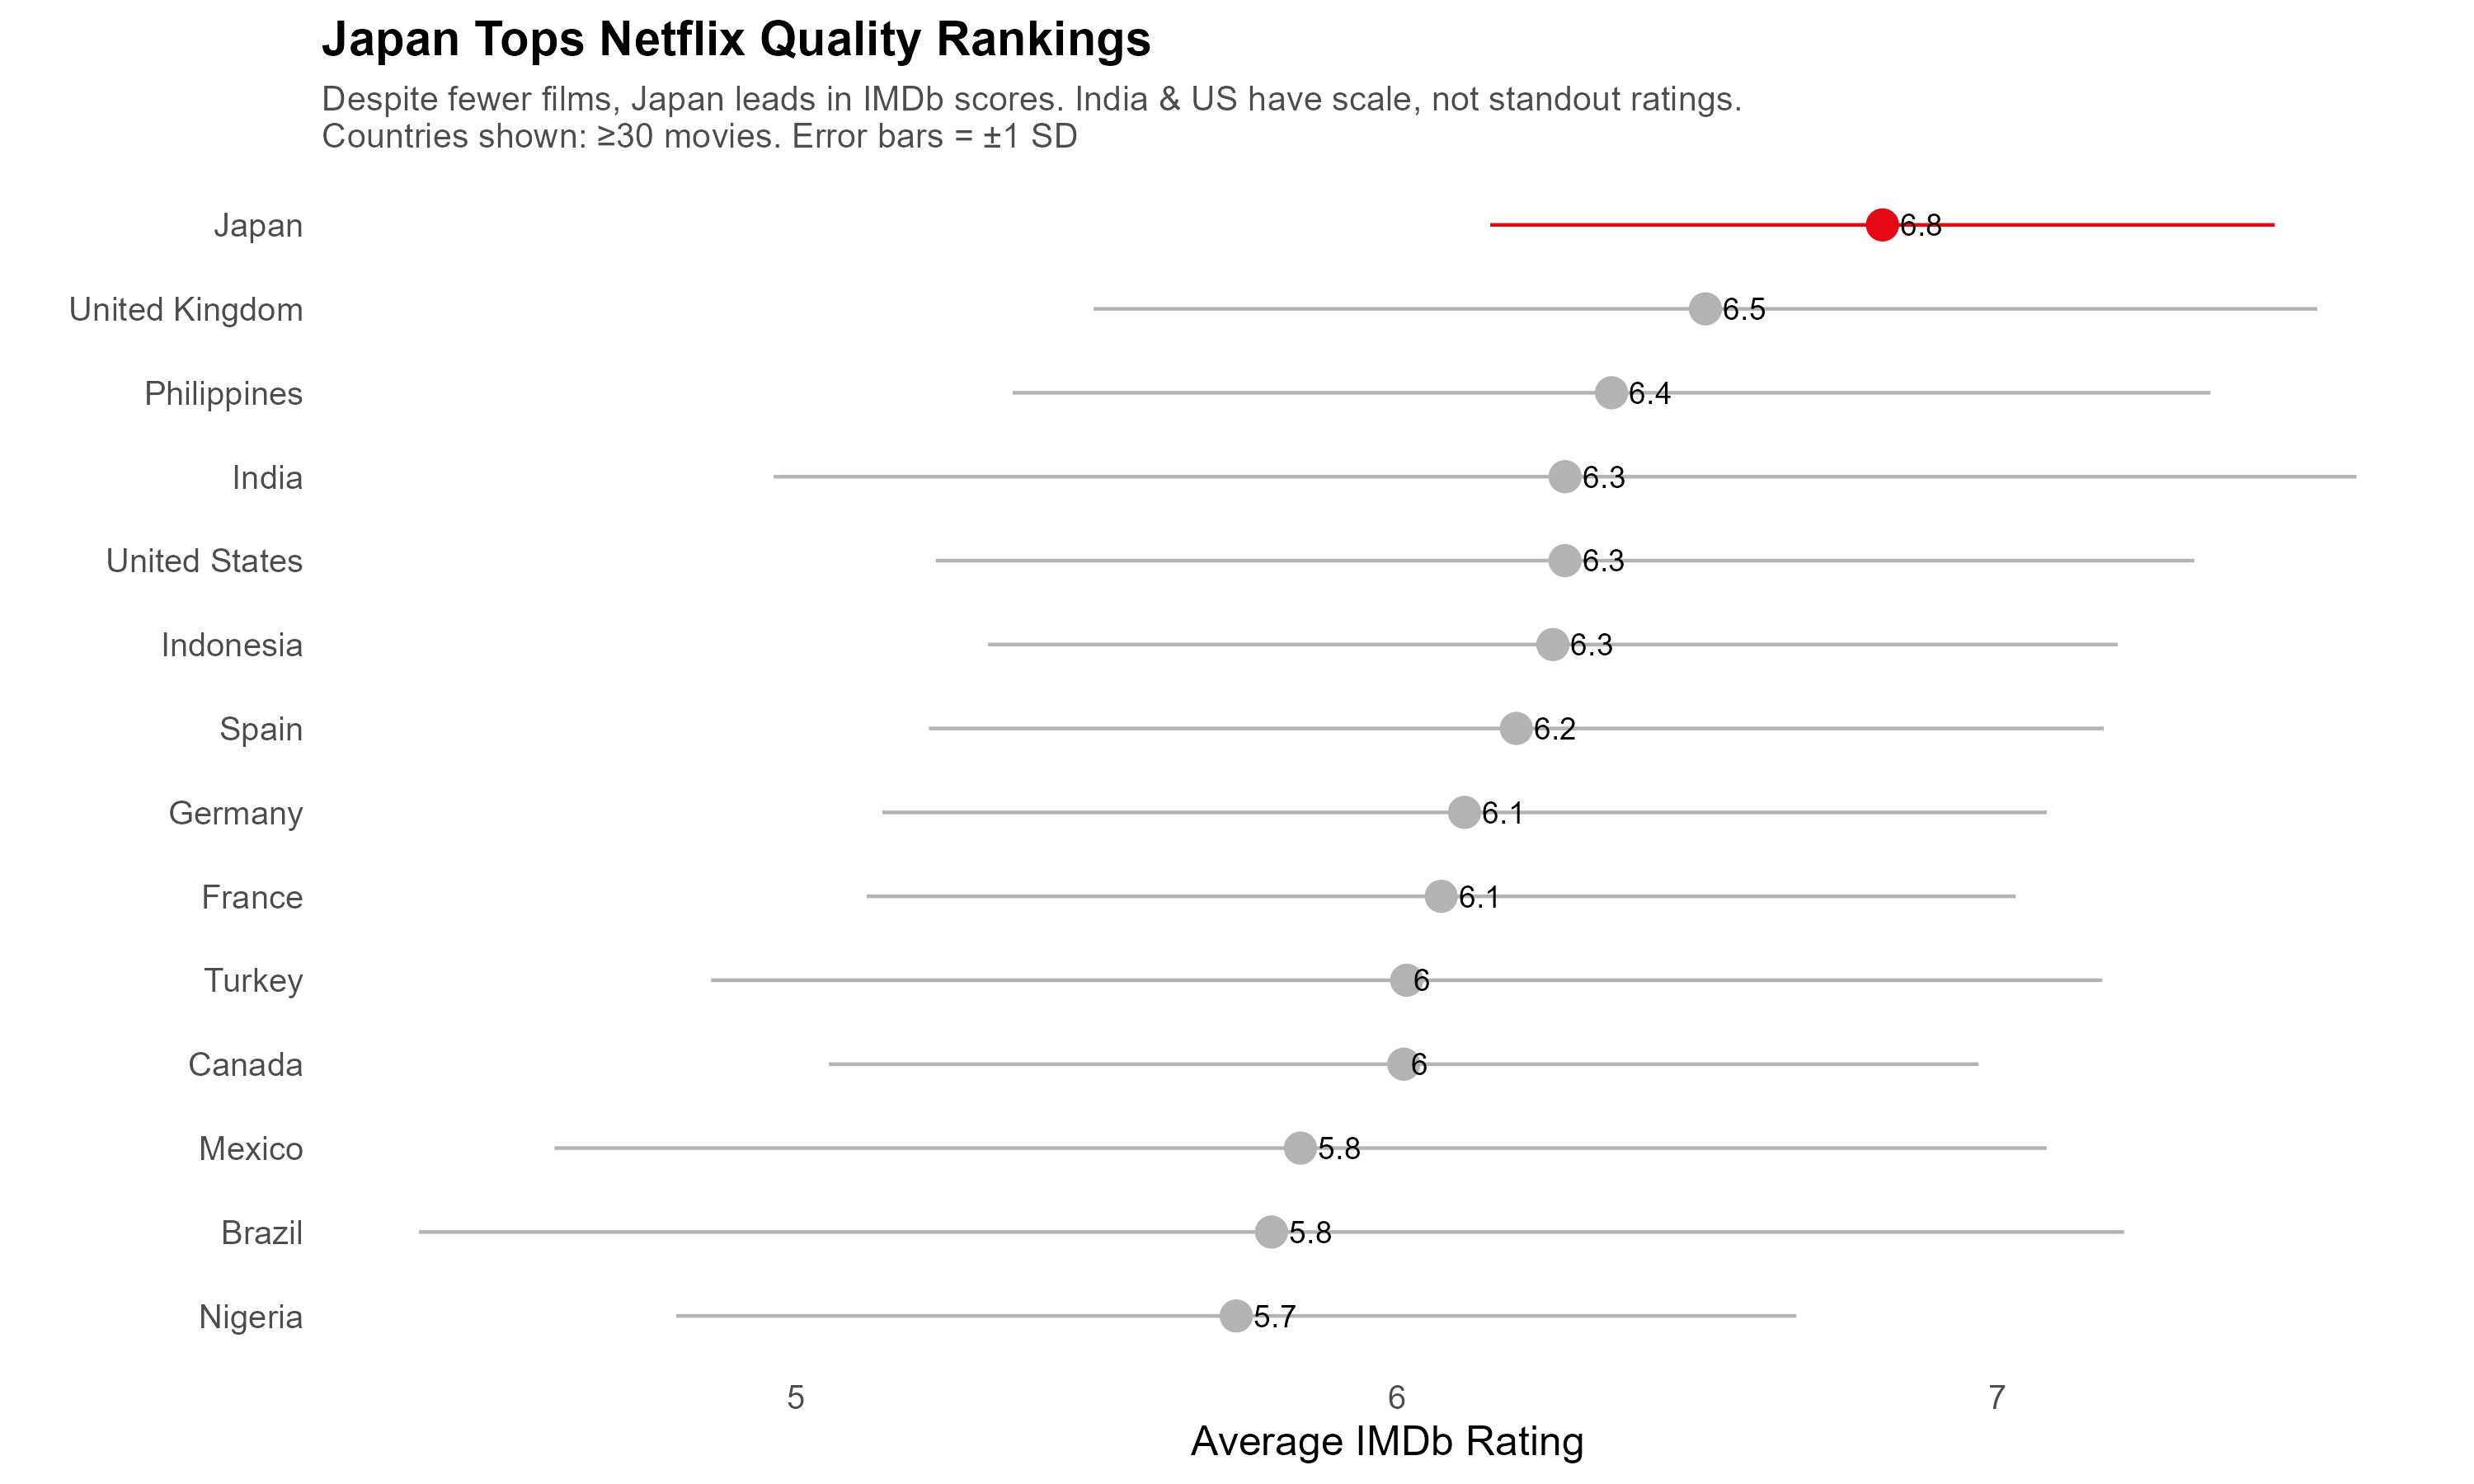
\includegraphics[width=0.9\linewidth]{../Question3/Results/countryrating} 

}

\caption{ }\label{fig:audienceengage-2}
\end{figure}
\begin{figure}

{\centering 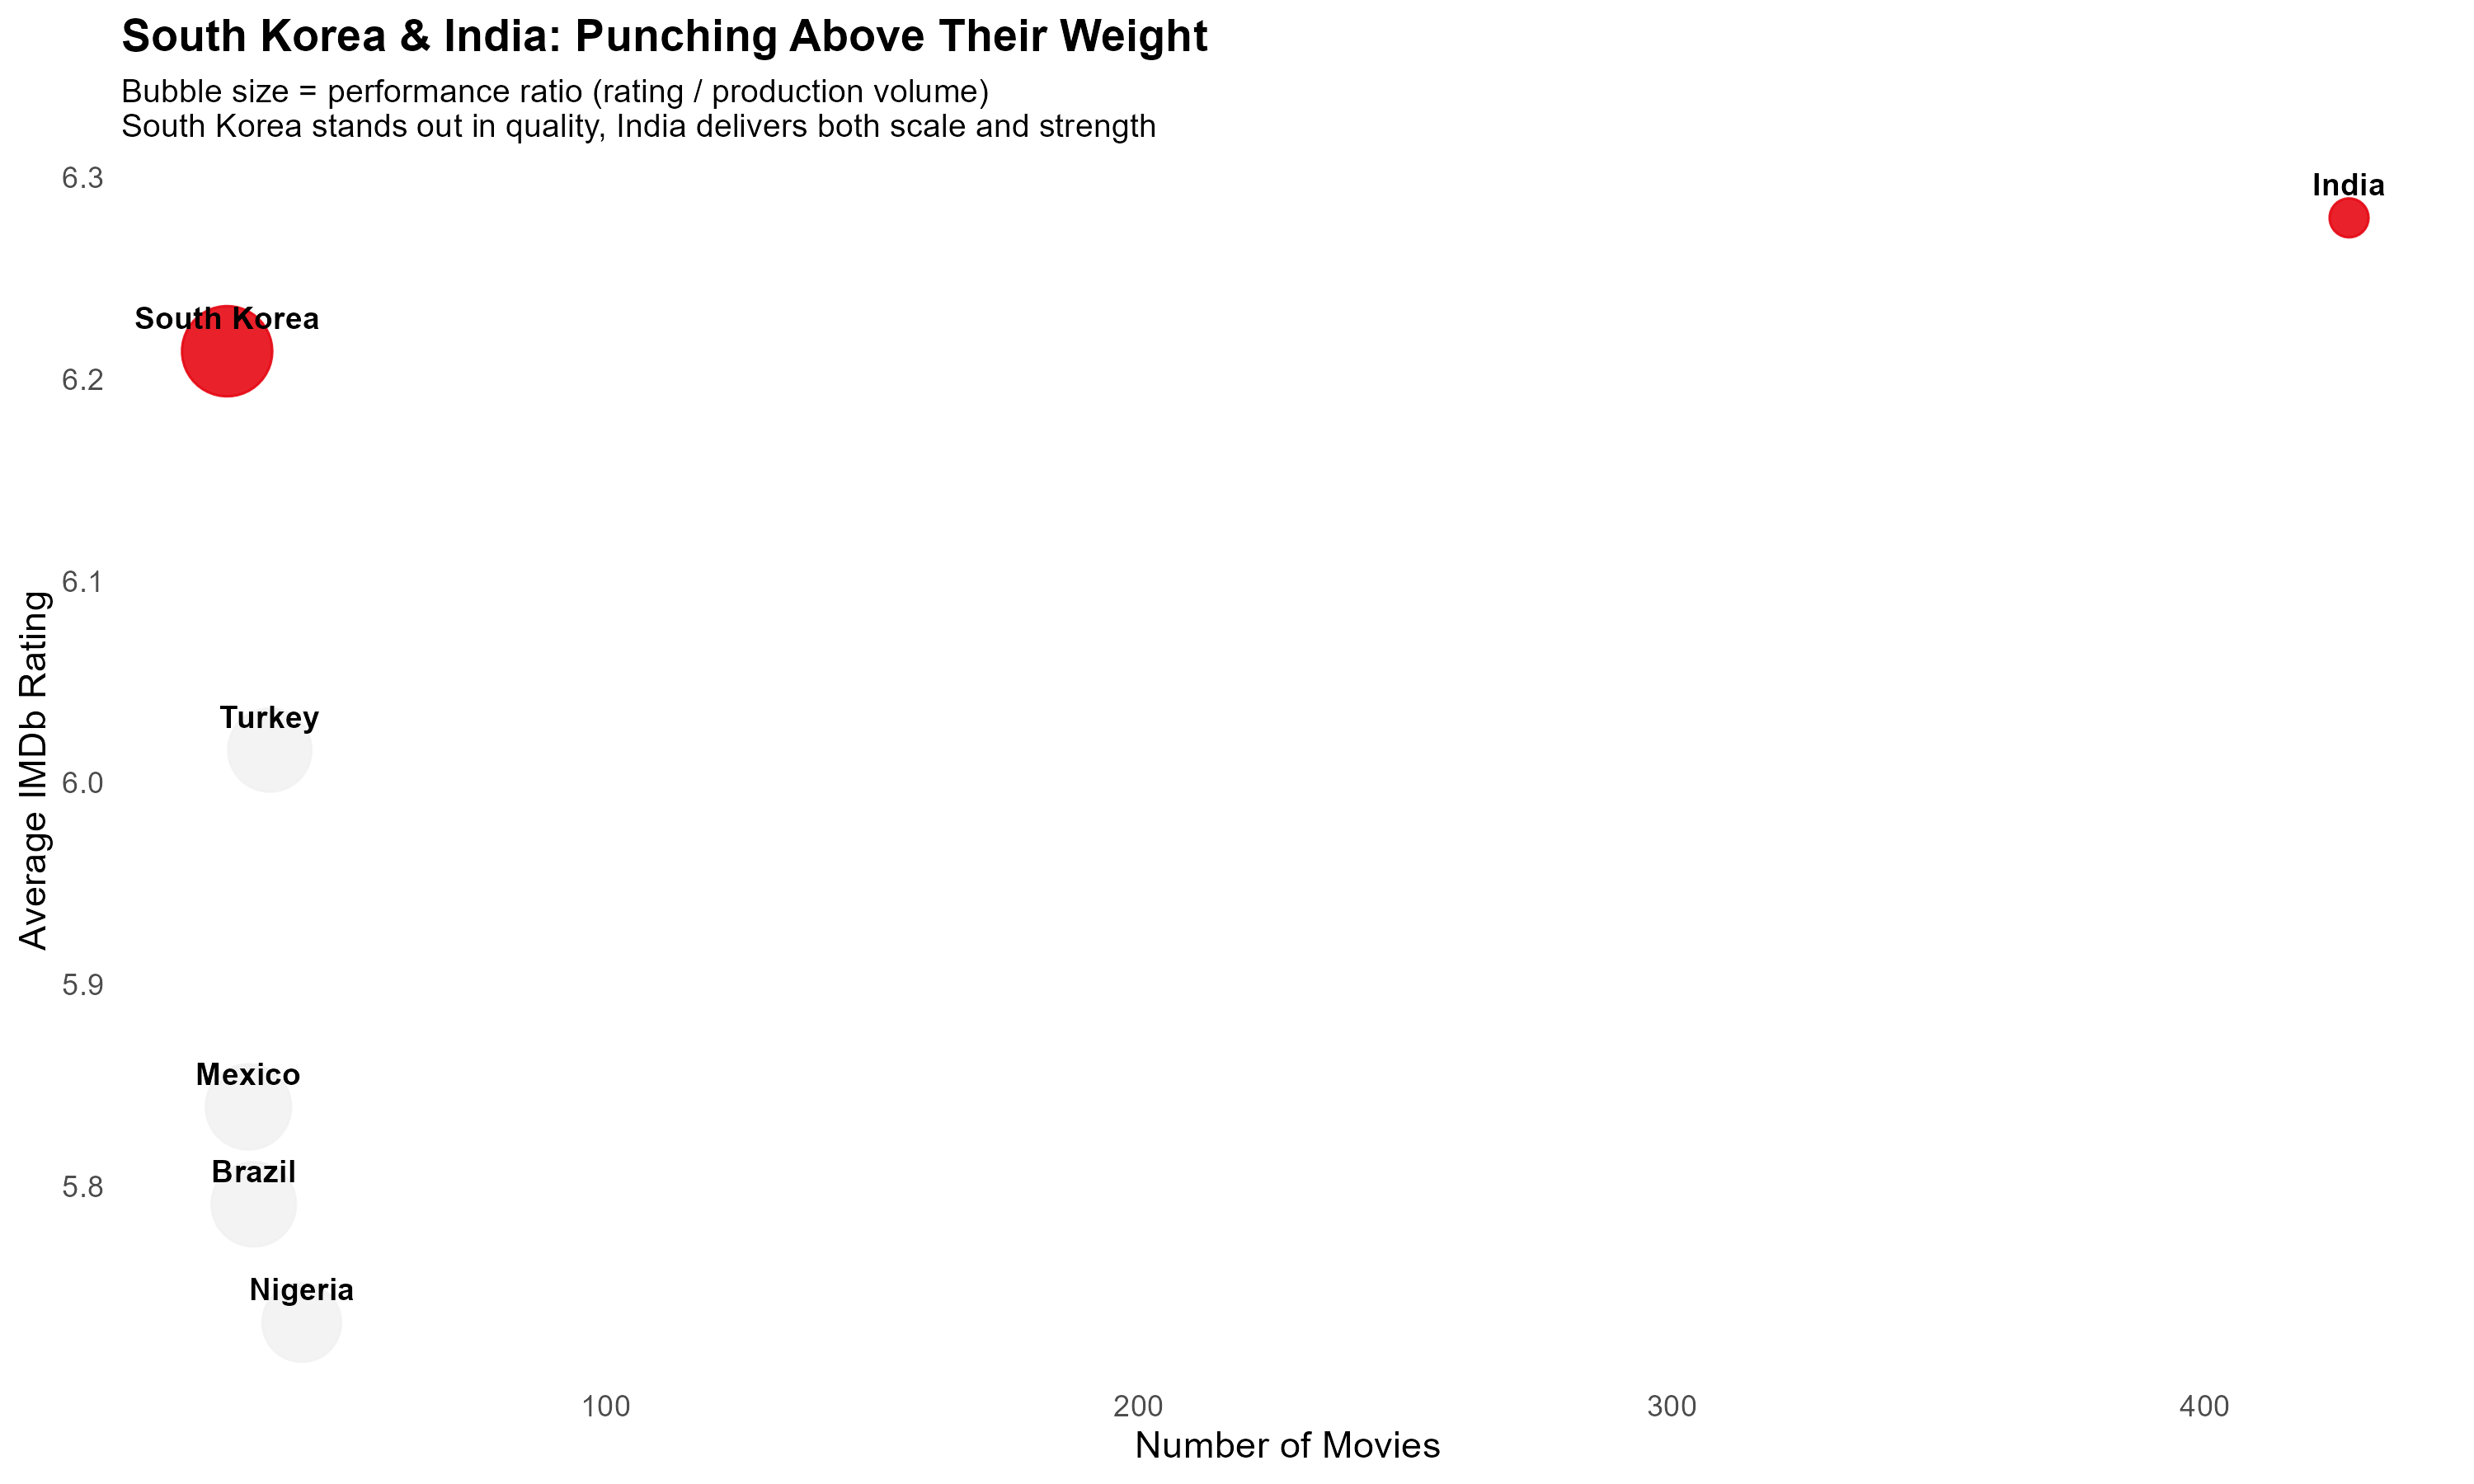
\includegraphics[width=0.9\linewidth]{../Question3/Results/emergers} 

}

\caption{ }\label{fig:audienceengage-3}
\end{figure}
\begin{figure}

{\centering 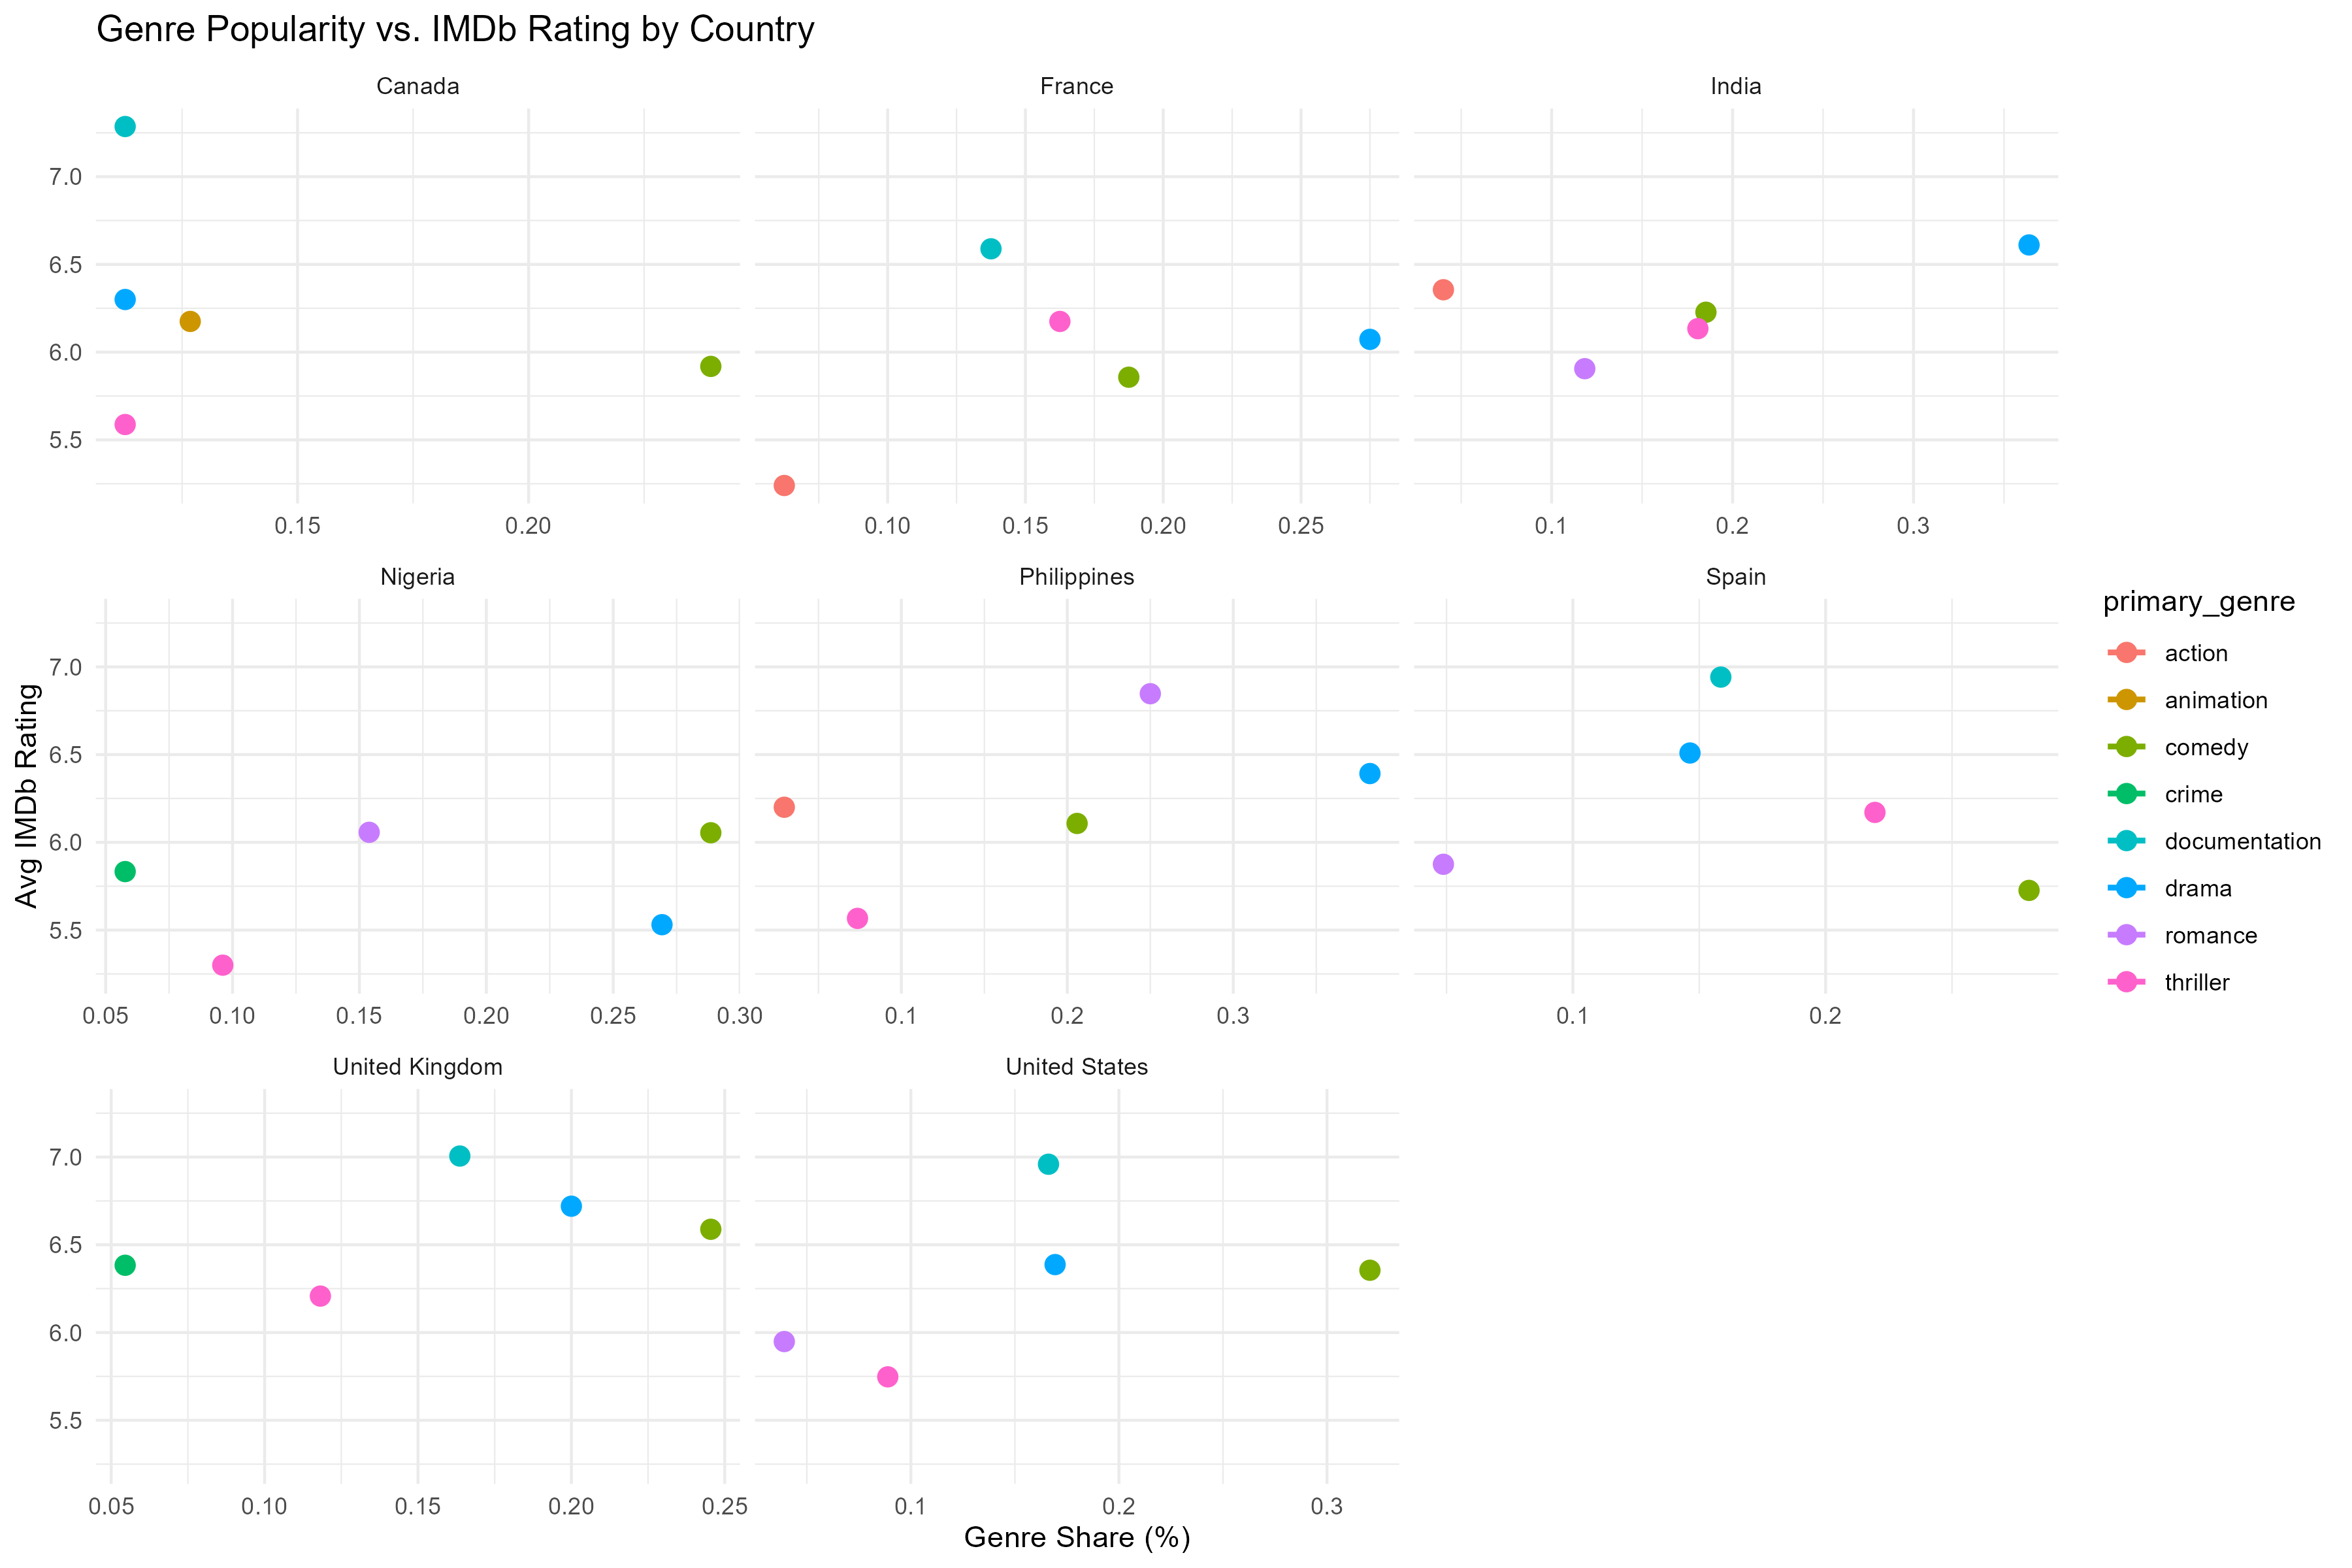
\includegraphics[width=0.9\linewidth]{../Question3/Results/genre_rating_plot} 

}

\caption{ }\label{fig:audienceengage-4}
\end{figure}
\begin{figure}

{\centering 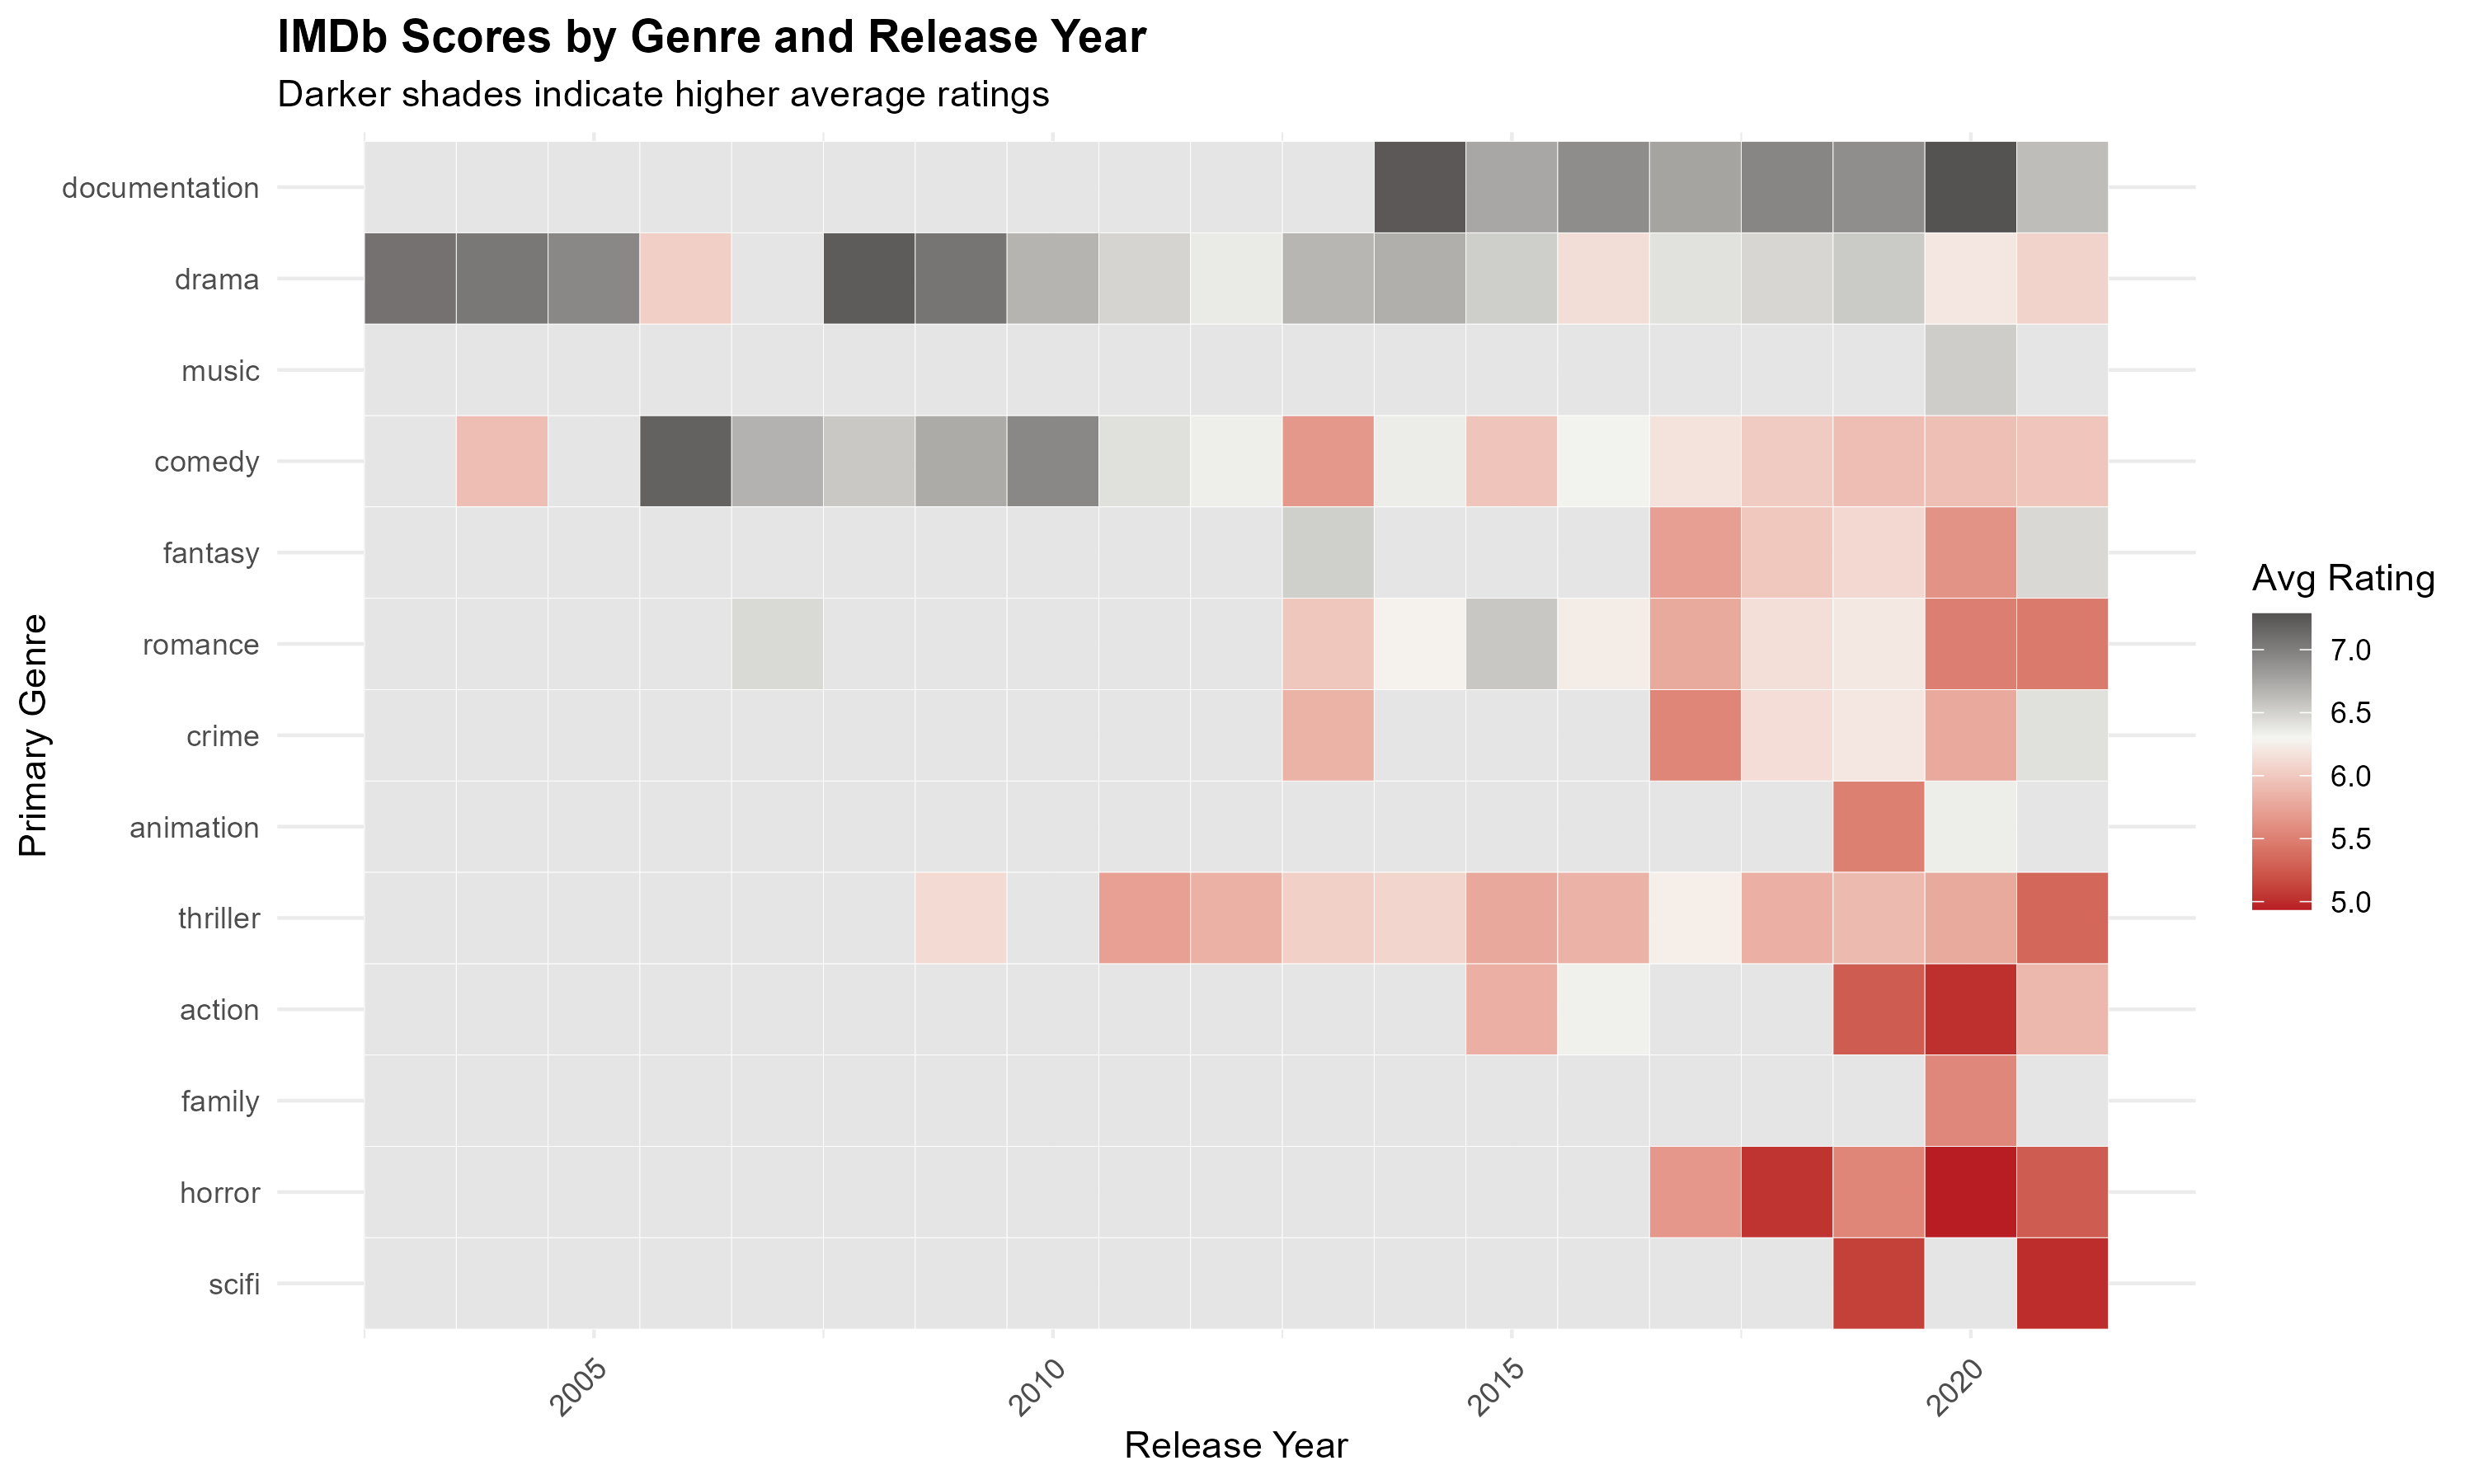
\includegraphics[width=0.9\linewidth]{../Question3/Results/genrescore} 

}

\caption{ }\label{fig:audienceengage-5}
\end{figure}
\begin{figure}

{\centering 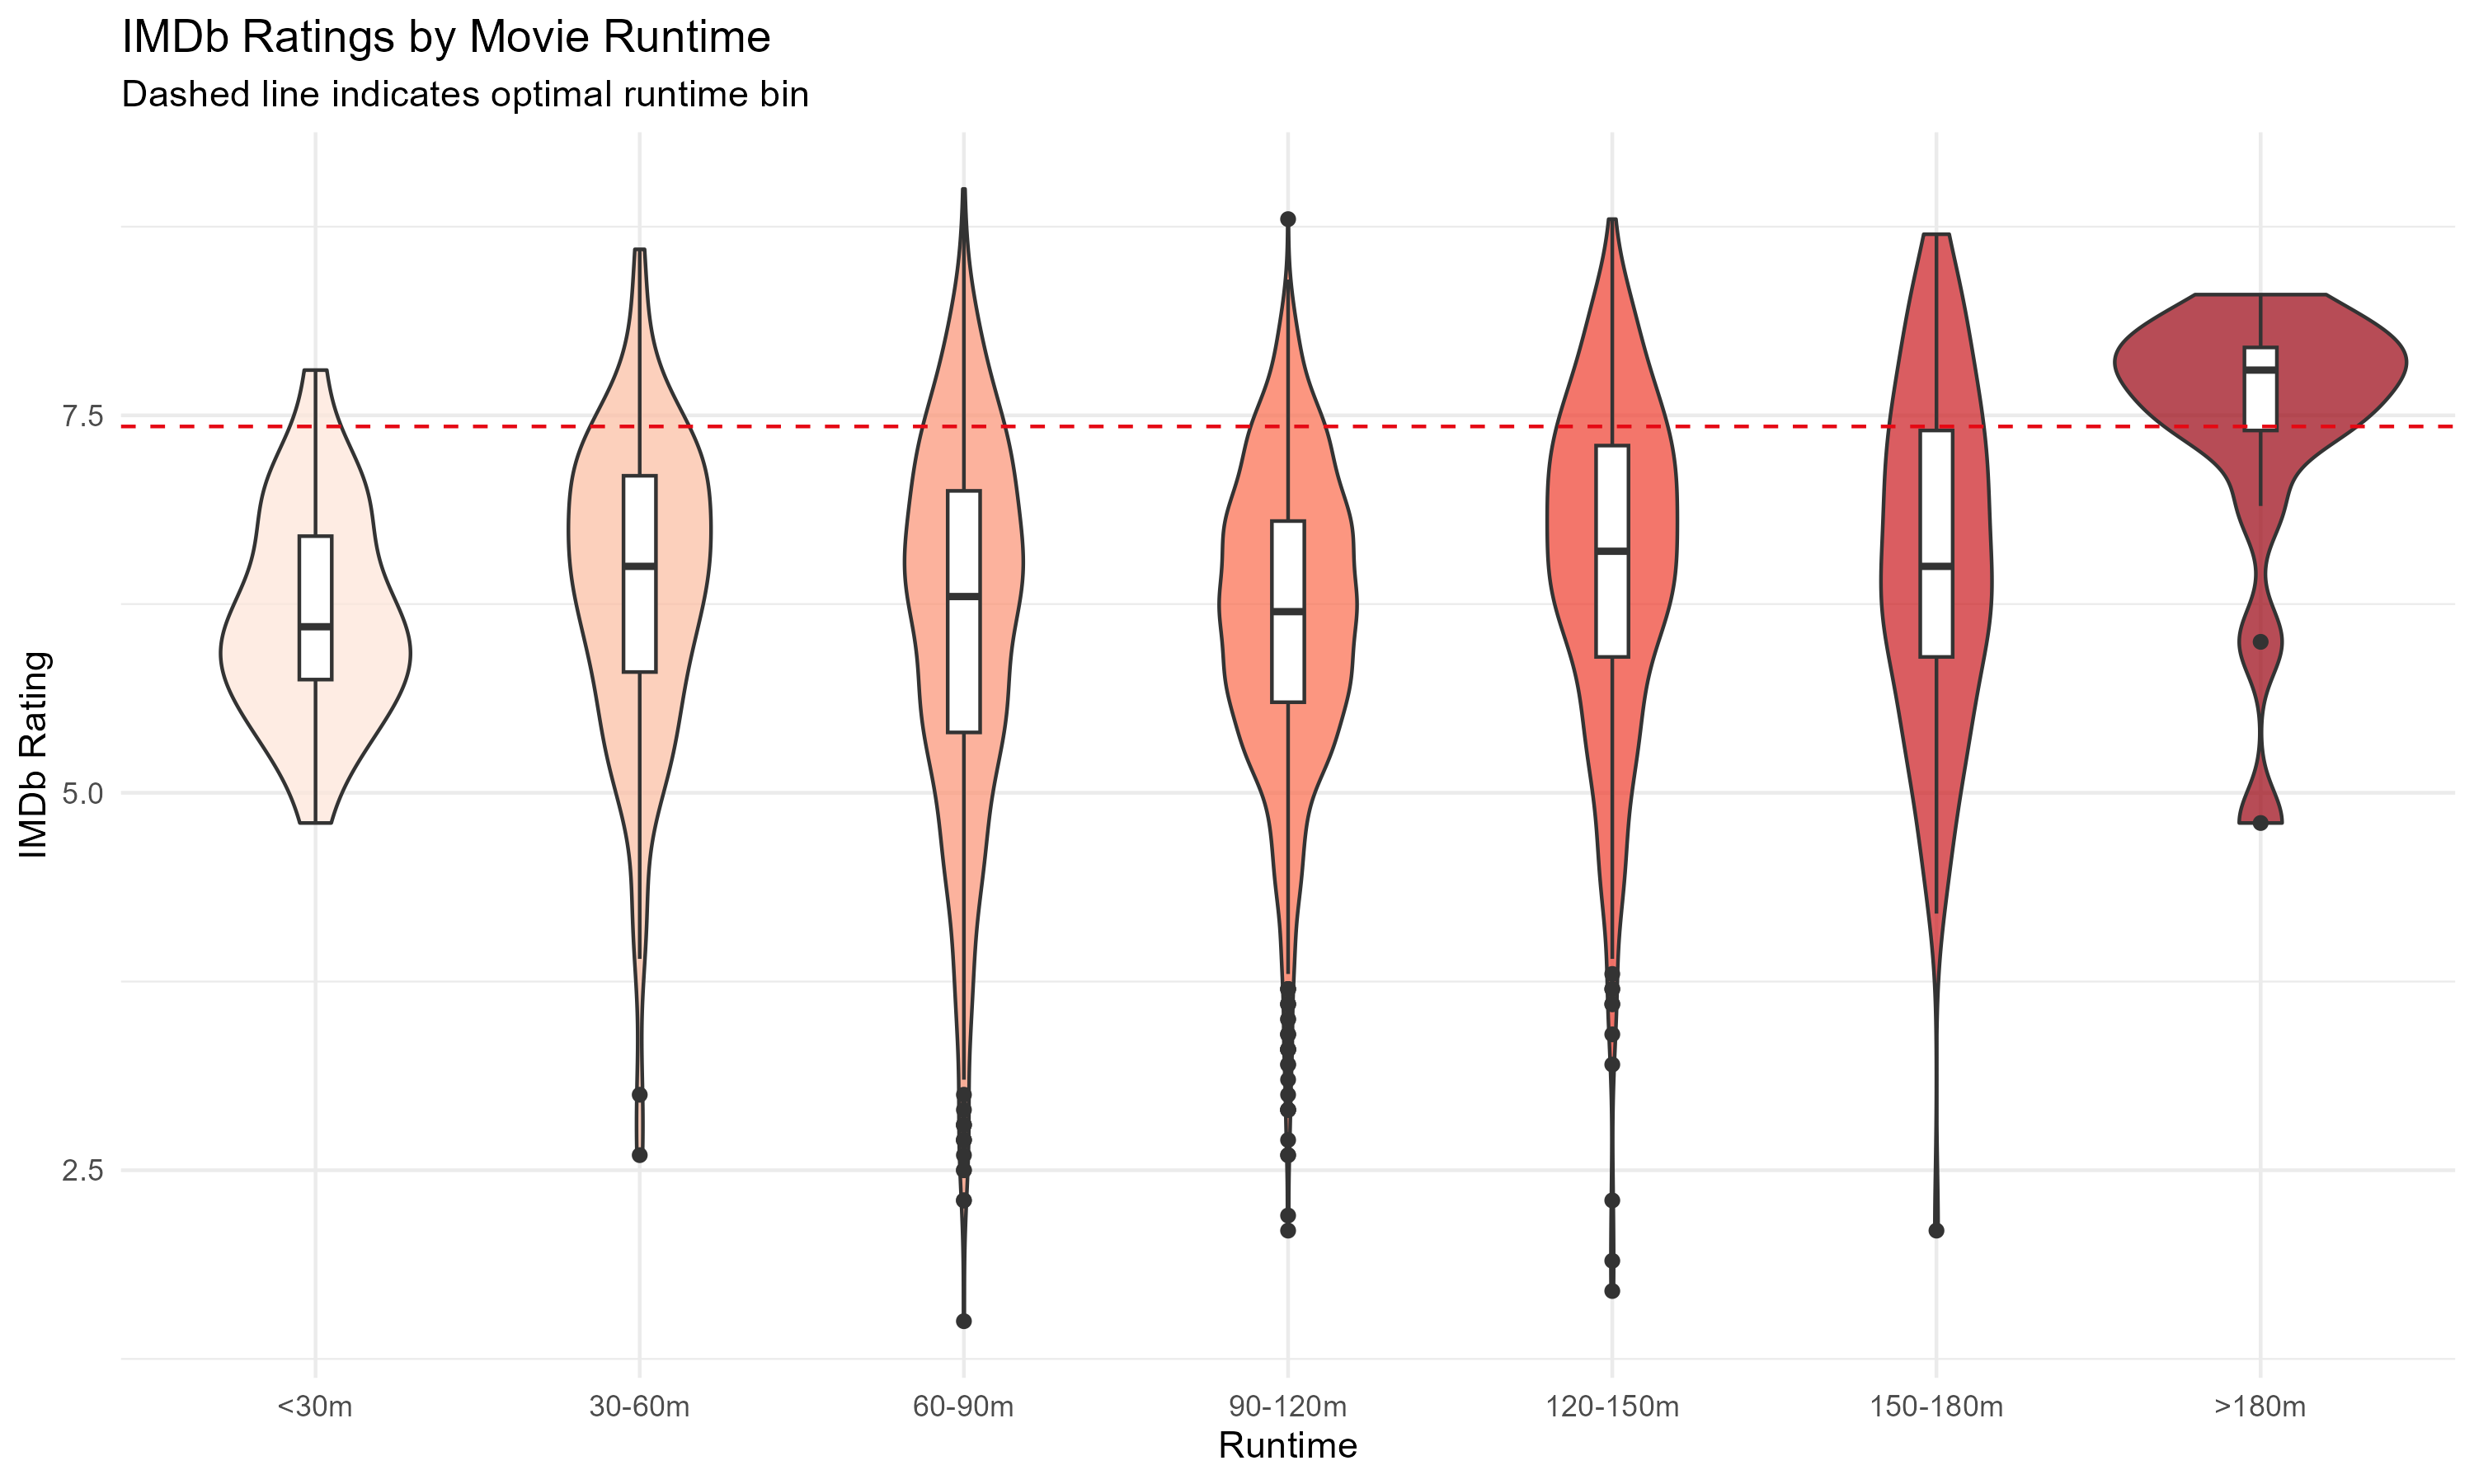
\includegraphics[width=0.9\linewidth]{../Question3/Results/IMDbratings} 

}

\caption{ }\label{fig:audienceengage-6}
\end{figure}
\begin{figure}

{\centering 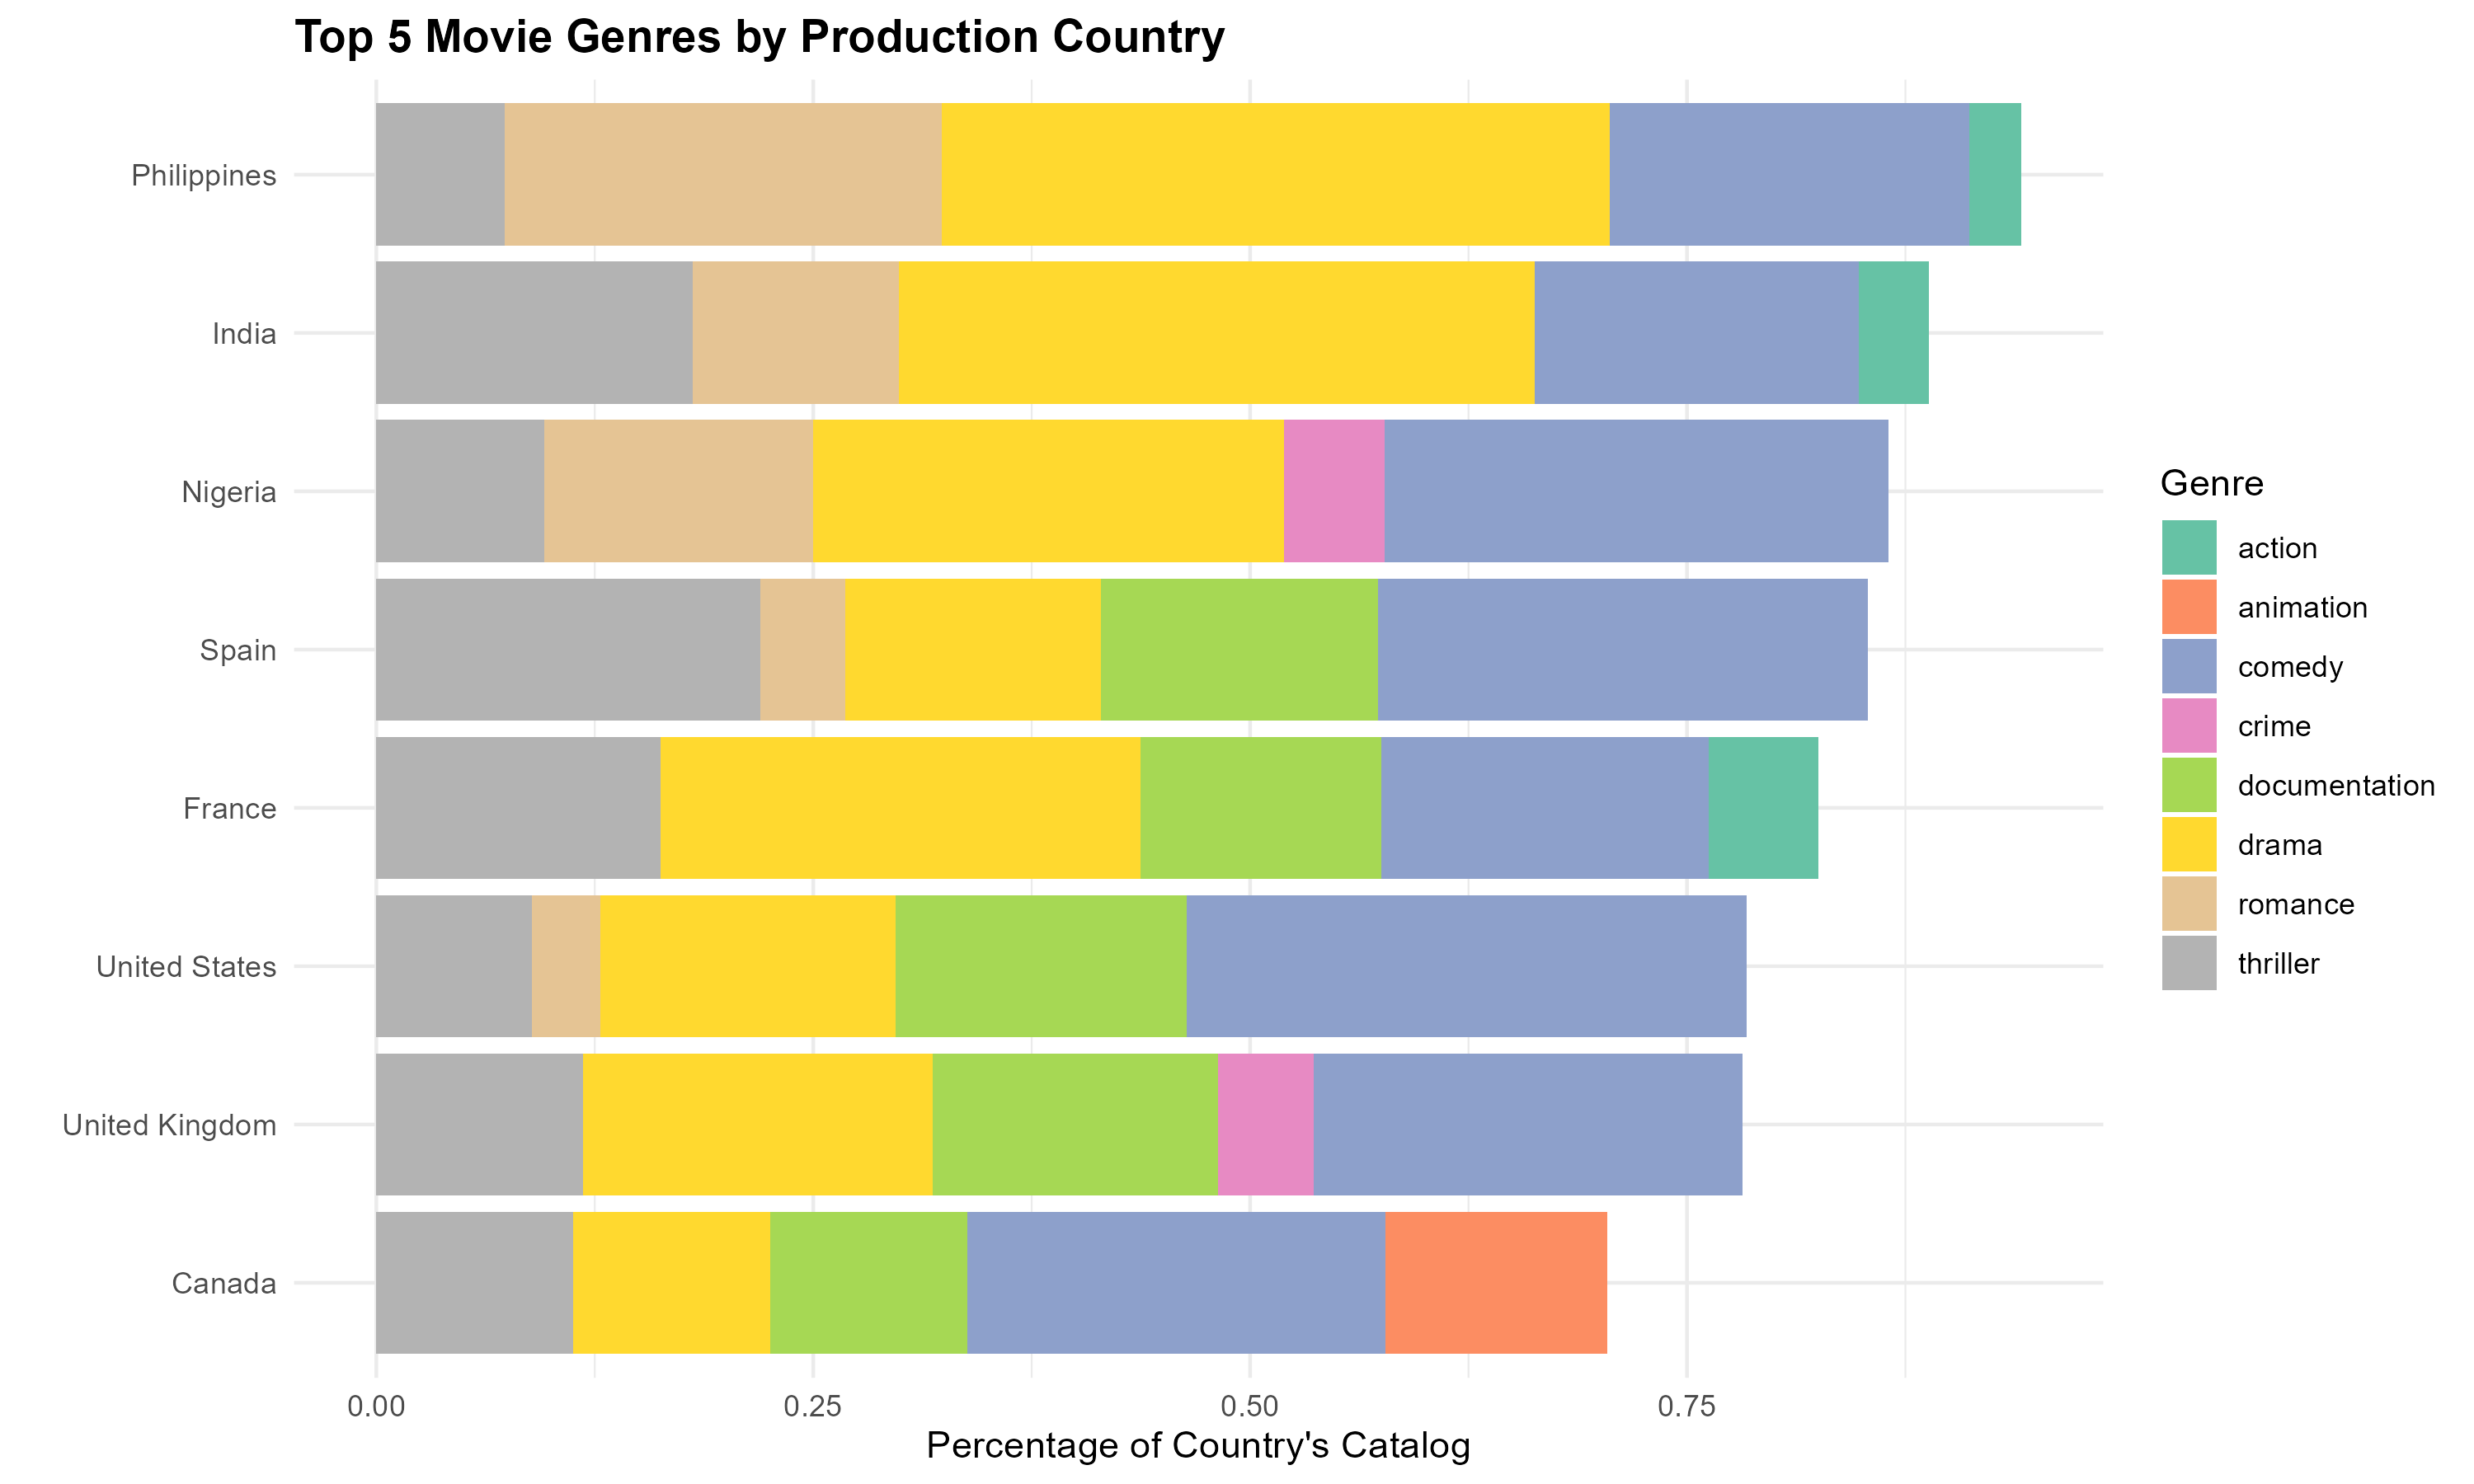
\includegraphics[width=0.9\linewidth]{../Question3/Results/top5movies} 

}

\caption{ }\label{fig:audienceengage-7}
\end{figure}
\begin{figure}

{\centering 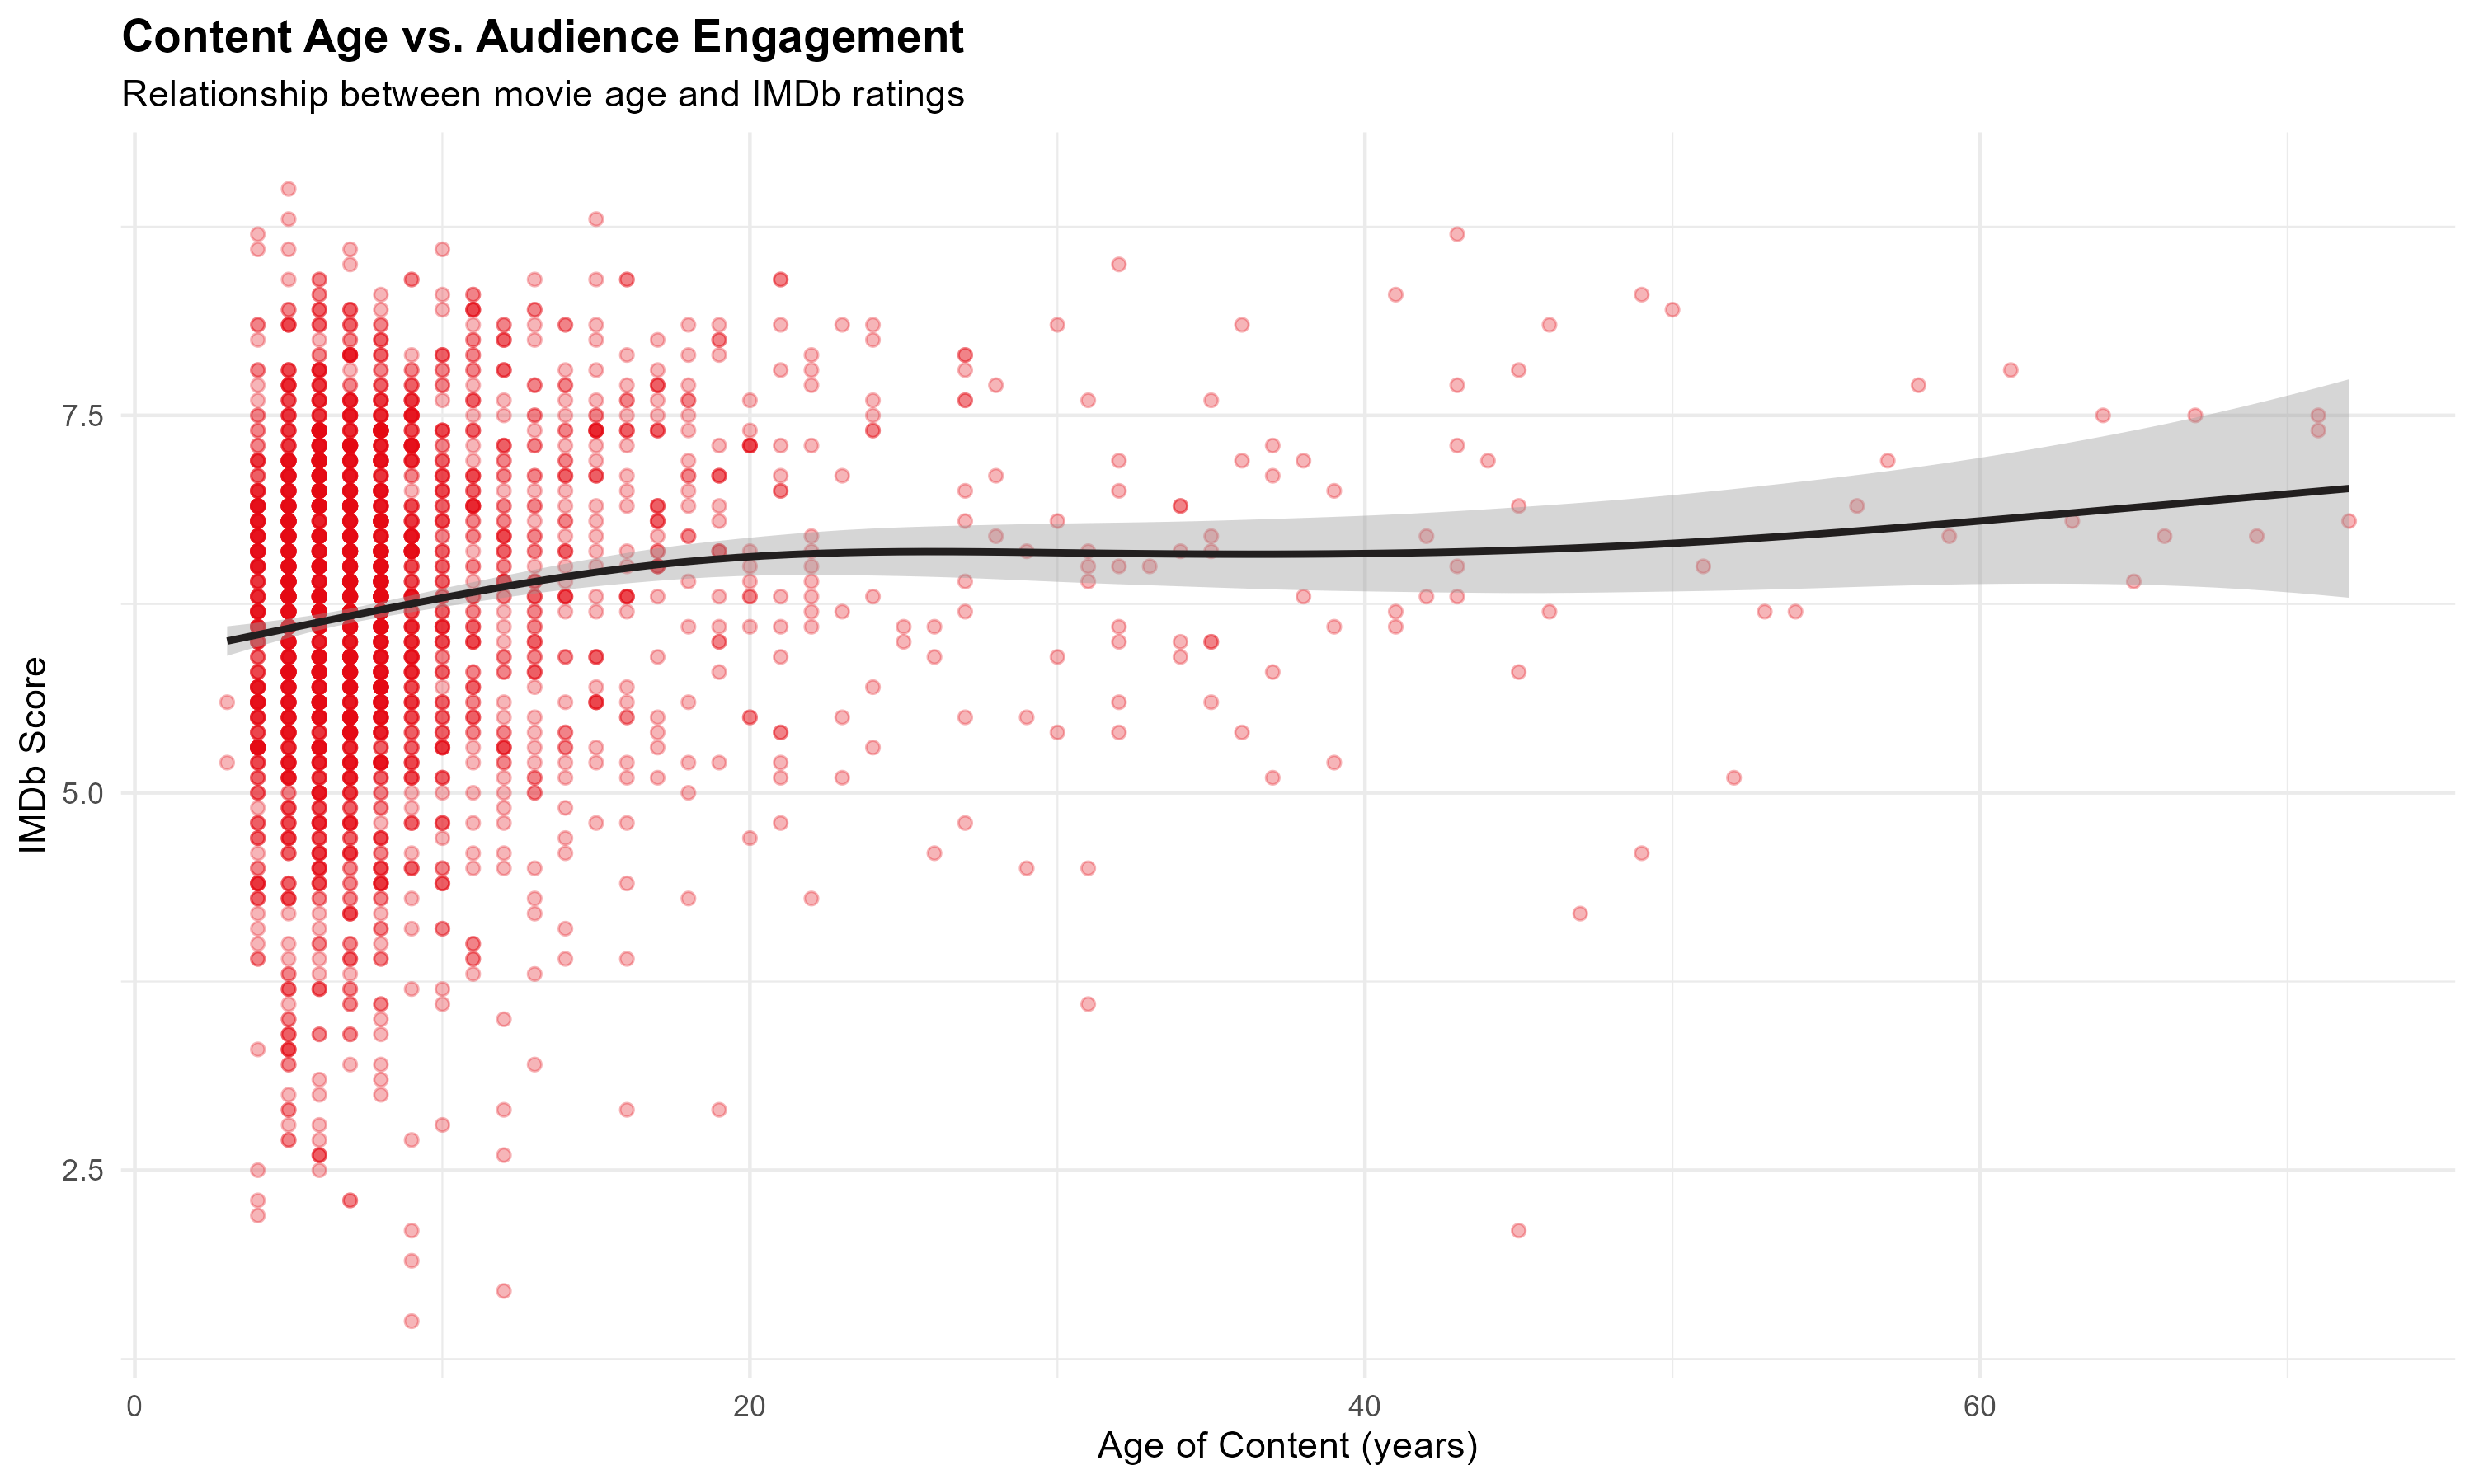
\includegraphics[width=0.9\linewidth]{../Question3/Results/viewership} 

}

\caption{ }\label{fig:audienceengage-8}
\end{figure}
\begin{figure}

{\centering 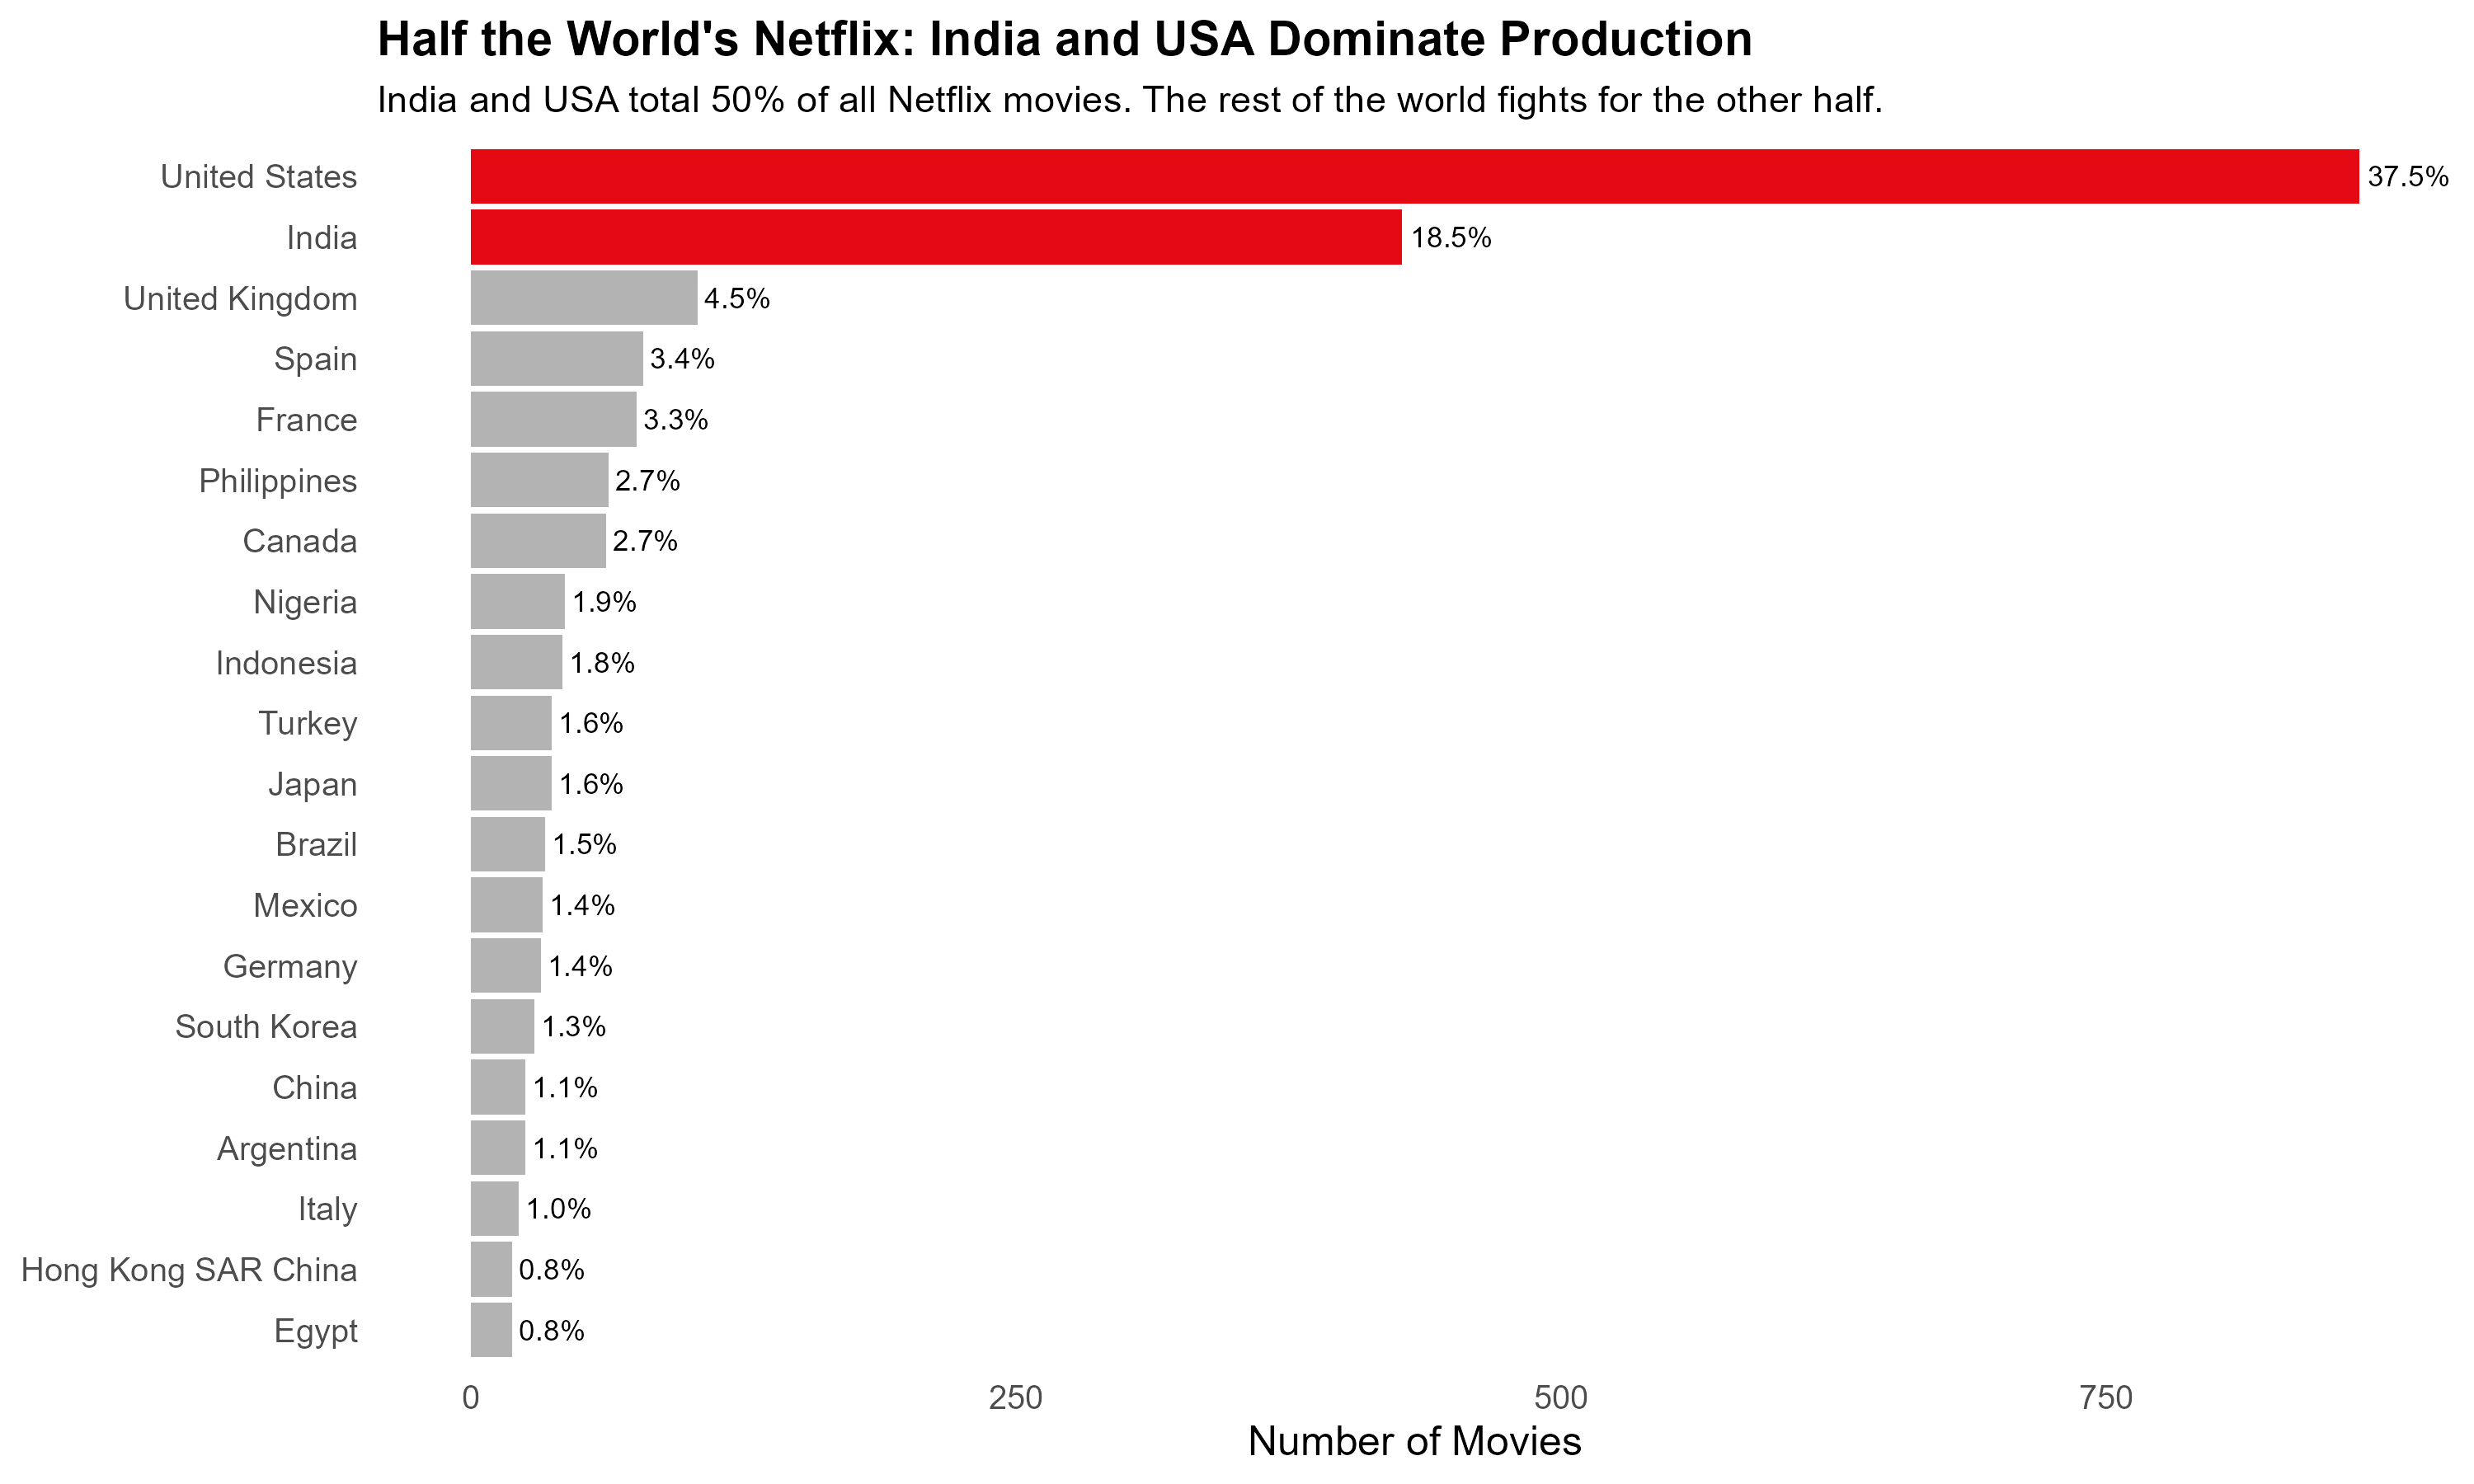
\includegraphics[width=0.9\linewidth]{../Question3/Results/top20creators} 

}

\caption{ }\label{fig:audienceengage-9}
\end{figure}

\subsection{Key Findings}\label{key-findings}

\subsubsection{1. Quality vs.~Volume Trade-Off}\label{quality-vs.-volume-trade-off}

Japanese titles, while constituting only 1.6\% of Netflix's catalogue, achieve superior average IMDb ratings (mean = 6.7, SD = ±0.3). By contrast, the United States and India collectively contribute over 50\% of Netflix's content but yield lower average ratings (mean = 6.1--6.3) (Figures 8, 15)
\textbf{Implication}: High-volume strategies may dilute perceived quality.

\subsubsection{2. Genre Performance Differentials}\label{genre-performance-differentials}

Content genres vary markedly in audience reception. Documentaries (mean = 7.6) and dramas (mean = 7.0) lead on quality metrics, while action and comedy lag behind (mean = 6.2 and 6.5 respectively) (Figure 11). Crime and thriller categories also demonstrate strong viewer engagement.

\textbf{Implication}:Narrative depth and authenticity drive audience satisfaction.

\subsubsection{3. Optimal Runtime Windows}\label{optimal-runtime-windows}

Ratings peak for films with runtimes between 90--120 minutes (mean = 7.5). Shorter or longer formats tend to correlate with lower ratings (Figure 12).
\textbf{Implication}:Viewer engagement is maximised within a standardised runtime threshold.

\subsubsection{4. Age and Longevity of Content}\label{age-and-longevity-of-content}

Older films (\textgreater20 years) sustain higher average ratings (mean = 8.5)(Figure 7) compared to recent productions (1--3 years; mean = 6.0)(Figure 14).
\textbf{Implication}:Legacy content benefits from curation and nostalgia; newer content faces saturation and discovery challenges.

\subsection{Strategic Recommendations for New Market Entrant}\label{strategic-recommendations-for-new-market-entrant}

To position competitively against incumbent platforms:

\subsubsection{1. Targeted Content Acquisition}\label{targeted-content-acquisition}

Prioritise \textbf{high-quality, underrepresented niches}---such as Japanese documentaries and international dramas---to differentiate on quality and build a prestige brand image.

\subsubsection{2. Genre Investment Strategy}\label{genre-investment-strategy}

Allocate production and licensing budgets towards \textbf{high-performing genres} (e.g., crime, thriller, drama). Avoid overserved categories like generic comedy unless uniquely positioned.

\subsubsection{3. Runtime Standardisation}\label{runtime-standardisation}

Anchor commissioned or licensed content within the 90--120 minute range to enhance user engagement and completion rates.

\subsection{Conclusion}\label{conclusion}

A differentiated, quality-first strategy that leverages genre insights, runtime discipline, and curated international content provides a clear pathway for new entrants to gain market share and investor confidence---without replicating the scale-driven pitfalls observed in Netflix's recent trajectory.

\#Question4 Billionaires

\subsection{Data analysis}\label{data-analysis}

We used R (Version 4.4.3; R Core Team, 2025) and the R-packages \emph{dplyr} (Version 1.1.4; Wickham, François, Henry, Müller, \& Vaughan, 2023), \emph{fastDummies} (Version 1.7.5; Kaplan, 2025), \emph{forcats} (Version 1.0.0; Wickham, 2023a), \emph{ggplot2} (Version 3.5.2; Wickham, 2016), \emph{ggrepel} (Version 0.9.6; Slowikowski, 2024), \emph{lubridate} (Version 1.9.4; Grolemund \& Wickham, 2011), \emph{papaja} (Version 0.1.3; Aust \& Barth, 2024), \emph{patchwork} (Version 1.3.0; Pedersen, 2024), \emph{purrr} (Version 1.0.4; Wickham \& Henry, 2025), \emph{readr} (Version 2.1.5; Wickham, Hester, \& Bryan, 2024), \emph{stringr} (Version 1.5.1; Wickham, 2023b), \emph{tibble} (Version 3.2.1; Müller \& Wickham, 2023), \emph{tidyr} (Version 1.3.1; Wickham, Vaughan, \& Girlich, 2024), \emph{tidyverse} (Version 2.0.0; Wickham et al., 2019), and \emph{tinylabels} (Version 0.2.5; Barth, 2025) for all our analyses.
\#\#Results

\#\#Discussion

\section{Question 5 Health}\label{question-5-health}

\subsection{On Air Script}\label{on-air-script}

For the 9-to-5 gamer: 1 hour of extra sleep beats 1 hour on the treadmill. Data shows stress-free living is your real cheat code.

We've been told for years to `exercise more'---but new data reveals the real game-changers: sleep and stress management. Here's the proof: Adults with poor sleep and high stress gained 7--10 pounds more than those with good sleep and low stress---based on regression analysis (p\textless0.01). The worst hit? Early-career professionals (ages 30--39), who saw up to 10 pounds more weight gain when stressed---even if they exercised. Why this matters: Gym memberships won't fix this. The solution? Protect your sleep: Aim for 7--9 hours, and keep a consistent schedule---it's your metabolic lifeline. Tame stress: Short walks, 5-minute breathing exercises, or setting work boundaries can slash health risks. Bottom line? Small changes to sleep and stress beat marathon workouts. Start tonight---your body will thank you.

\begin{figure}
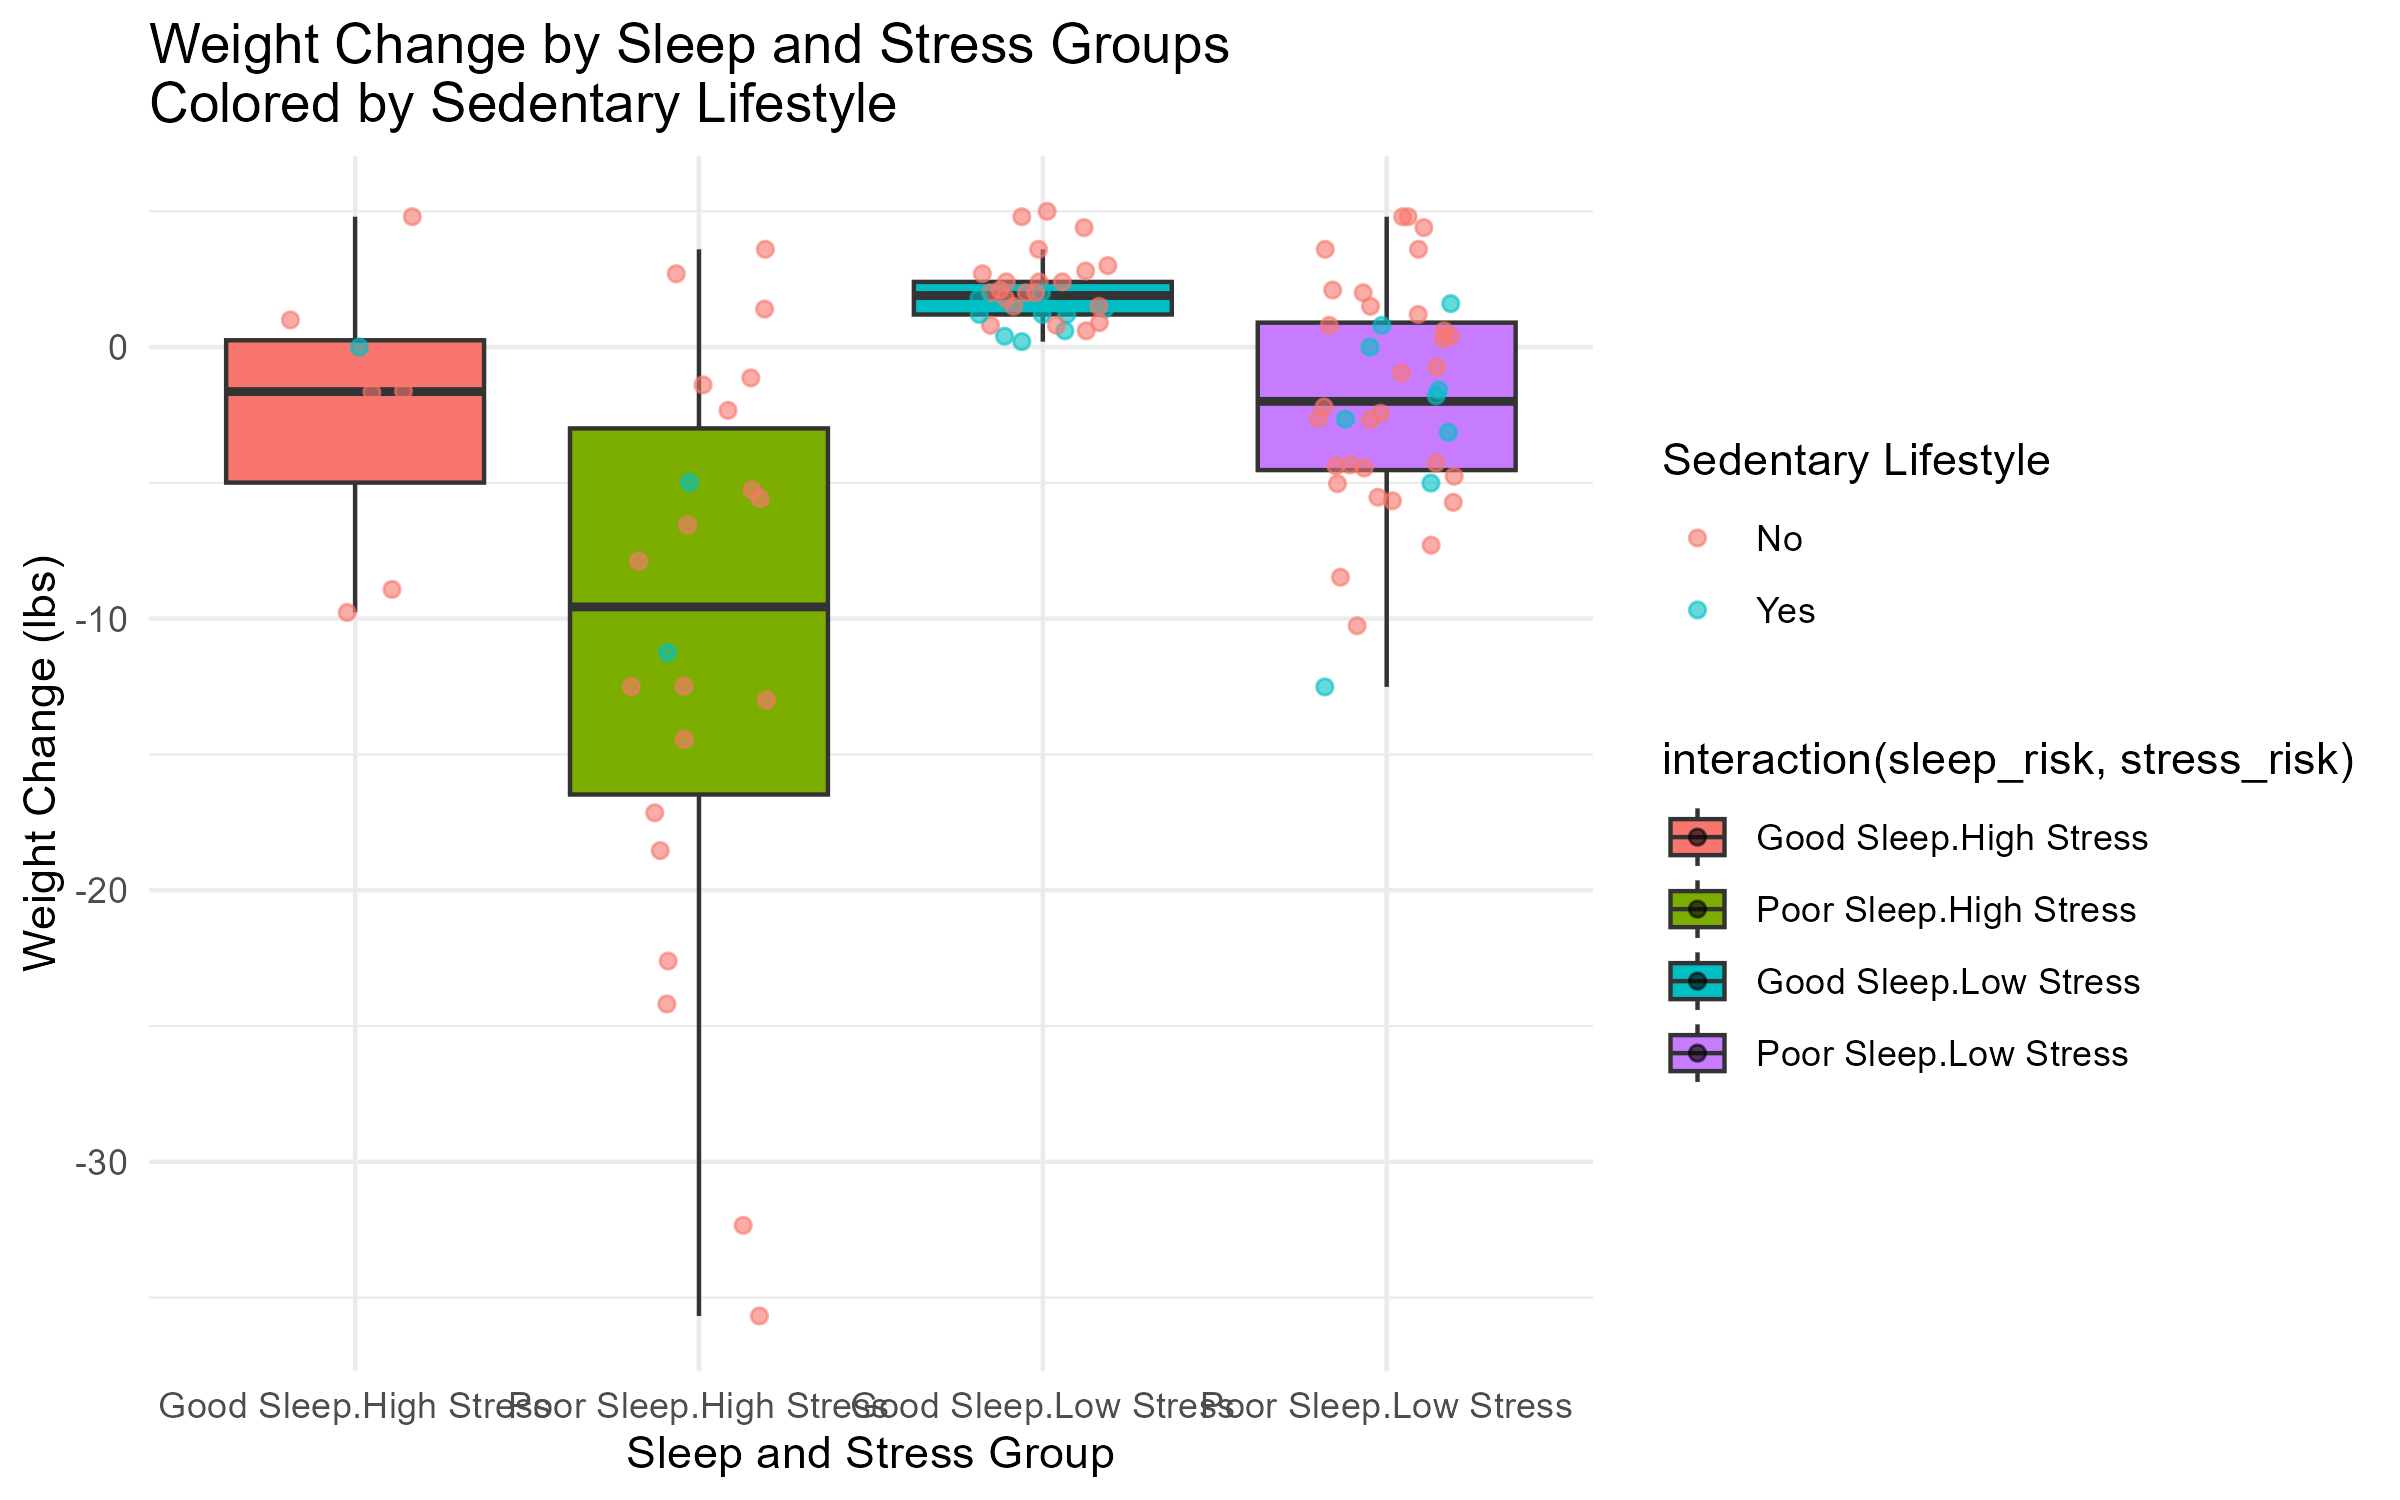
\includegraphics[width=0.9\linewidth]{../Question5/Results/Sleep_Stress_Boxplot} \caption{ }\label{fig:sleep-stress-boxplot}
\end{figure}

\begin{table}

\caption{(\#tab:sleep-risk-pivot )Weight Change Summary}
\centering
\begin{tabular}[t]{l|l|r|r|r}
\hline
Gender & age\_group & mean\_weight\_change & median\_weight\_change & n\\
\hline
F & Adults (20-29) & -1.0181151 & -0.3680584 & 10\\
\hline
F & Early Career (30-39) & -2.4545587 & -1.3943583 & 11\\
\hline
F & Middle-aged (40-49) & -3.4805916 & 0.7000000 & 12\\
\hline
F & Preretirement (50-64) & -1.5639095 & 0.0000000 & 9\\
\hline
F & Teenagers (<20) & -1.7940640 & -1.7940640 & 1\\
\hline
M & Adults (20-29) & -2.3794779 & -0.1679132 & 14\\
\hline
M & Early Career (30-39) & -5.5847844 & 0.6000000 & 12\\
\hline
M & Middle-aged (40-49) & -3.7051828 & 0.4500000 & 12\\
\hline
M & Preretirement (50-64) & -0.8648233 & -0.3807078 & 14\\
\hline
M & Teenagers (<20) & -5.2528414 & -5.7184960 & 5\\
\hline
\end{tabular}
\end{table}

\begin{table}

\caption{(\#tab:sleep-risk-pivot )Sleep Risk Pivot Summary}
\centering
\begin{tabular}[t]{l|l|r|r}
\hline
Poor Sleep Risk & age\_group & Mean\_Weight\_Change & Count\\
\hline
No & Adults (20-29) & 0.2142665 & 9\\
\hline
No & Early Career (30-39) & 1.5777778 & 9\\
\hline
No & Middle-aged (40-49) & 2.9571429 & 7\\
\hline
No & Preretirement (50-64) & -0.0982816 & 11\\
\hline
No & Teenagers (<20) & 1.9500000 & 2\\
\hline
Yes & Adults (20-29) & -3.0281494 & 15\\
\hline
Yes & Early Career (30-39) & -7.7298256 & 14\\
\hline
Yes & Middle-aged (40-49) & -6.2899584 & 17\\
\hline
Yes & Preretirement (50-64) & -2.0918011 & 12\\
\hline
Yes & Teenagers (<20) & -7.9895678 & 4\\
\hline
\end{tabular}
\end{table}

\begin{table}

\caption{(\#tab:sleep-risk-pivot )Stress Risk Pivot Summary}
\centering
\begin{tabular}[t]{l|l|r|r}
\hline
Poor Sleep Risk & age\_group & Mean\_Weight\_Change & Count\\
\hline
No & Adults (20-29) & 0.2142665 & 9\\
\hline
No & Early Career (30-39) & 1.5777778 & 9\\
\hline
No & Middle-aged (40-49) & 2.9571429 & 7\\
\hline
No & Preretirement (50-64) & -0.0982816 & 11\\
\hline
No & Teenagers (<20) & 1.9500000 & 2\\
\hline
Yes & Adults (20-29) & -3.0281494 & 15\\
\hline
Yes & Early Career (30-39) & -7.7298256 & 14\\
\hline
Yes & Middle-aged (40-49) & -6.2899584 & 17\\
\hline
Yes & Preretirement (50-64) & -2.0918011 & 12\\
\hline
Yes & Teenagers (<20) & -7.9895678 & 4\\
\hline
\end{tabular}
\end{table}

\newpage

\begin{longtable}[]{@{}
  >{\raggedright\arraybackslash}p{(\linewidth - 4\tabcolsep) * \real{0.5138}}
  >{\raggedright\arraybackslash}p{(\linewidth - 4\tabcolsep) * \real{0.2477}}
  >{\raggedright\arraybackslash}p{(\linewidth - 4\tabcolsep) * \real{0.2294}}@{}}
\toprule\noalign{}
\begin{minipage}[b]{\linewidth}\raggedright
\end{minipage} & \begin{minipage}[b]{\linewidth}\raggedright
Sleep-Stress Interaction
\end{minipage} & \begin{minipage}[b]{\linewidth}\raggedright
Stress-Age Interaction
\end{minipage} \\
\midrule\noalign{}
\endhead
\midrule\noalign{}
\multicolumn{3}{@{}>{\raggedright\arraybackslash}p{(\linewidth - 4\tabcolsep) * \real{0.9908} + 4\tabcolsep}@{}}{%
\begin{minipage}[t]{\linewidth}\raggedright
\begin{itemize}
\tightlist
\item
  p \textless{} 0.1, ** p \textless{} 0.05, *** p \textless{} 0.01
\end{itemize}
\end{minipage}} \\
\bottomrule\noalign{}
\endlastfoot
(Intercept) & 1.758 & -0.315 \\
& (6.660) & (1.510) \\
sleep\_riskPoor Sleep & -7.168*** & \\
& (2.704) & \\
stress\_riskLow Stress & 5.800** & \\
& (2.717) & \\
physical\_activityModerately Active & -1.142 & \\
& (1.893) & \\
physical\_activitySedentary & -0.539 & \\
& (1.982) & \\
physical\_activityVery Active & -1.076 & \\
& (2.311) & \\
age\_groupEarly Career (30-39) & -2.976 & 0.653 \\
& (1.875) & (2.135) \\
age\_groupMiddle-aged (40-49) & -2.226 & 0.107 \\
& (1.766) & (2.103) \\
age\_groupPreretirement (50-64) & -0.777 & 0.164 \\
& (1.891) & (2.135) \\
age\_groupTeenagers (\textless20) & -3.178 & -1.867 \\
& (2.861) & (3.094) \\
GenderM & -1.650 & \\
& (1.597) & \\
Daily Caloric Surplus/Deficit & 0.002 & \\
& (0.003) & \\
BMR (Calories) & -0.001 & \\
& (0.002) & \\
Duration (weeks) & -0.158 & \\
& (0.175) & \\
sleep\_riskPoor Sleep × stress\_riskLow Stress & 2.980 & \\
& (3.290) & \\
High Stress RiskYes & & -4.493* \\
& & (2.615) \\
High Stress RiskYes × age\_groupEarly Career (30-39) & & -10.049*** \\
& & (3.785) \\
High Stress RiskYes × age\_groupMiddle-aged (40-49) & & -7.112* \\
& & (3.767) \\
\multicolumn{3}{@{}>{\raggedright\arraybackslash}p{(\linewidth - 4\tabcolsep) * \real{0.9908} + 4\tabcolsep}@{}}{%
High Stress RiskYes × age\_groupPreretirement (50-64) \textbar{} \textbar{} 1.248 \textbar{}} \\
& & (3.785) \\
High Stress RiskYes × age\_groupTeenagers (\textless20) & & -10.476 \\
& & (7.112) \\
Num.Obs. & 100 & 100 \\
R2 & 0.455 & 0.402 \\
R2 Adj. & 0.366 & 0.342 \\
AIC & 655.5 & 654.9 \\
BIC & 697.2 & 683.5 \\
Log.Lik. & -311.752 & -316.433 \\
RMSE & 5.47 & 5.73 \\
\end{longtable}

\subsubsection{\texorpdfstring{\textbf{Key Findings on Health Determinants}}{Key Findings on Health Determinants}}\label{key-findings-on-health-determinants}

\begin{enumerate}
\def\labelenumi{\arabic{enumi}.}
\tightlist
\item
  \textbf{Sleep Quality is Critical}:

  \begin{itemize}
  \tightlist
  \item
    Poor sleep correlates with \textbf{-7.2 lbs} weight gain (\emph{p\textless0.01}), surpassing the impact of physical activity (non-significant coefficients).\\
  \item
    Teens and early-career adults with poor sleep show the worst outcomes (\textbf{-7.7 to -8.0 lbs} mean weight change).Teens are abstracted from main analysis as their n is very small , n =5 .
  \end{itemize}
\item
  \textbf{Stress Drives Negative Outcomes}:

  \begin{itemize}
  \tightlist
  \item
    High stress alone leads to \textbf{-4.5 lbs} weight gain (\emph{p\textless0.1}).\\
  \item
    Stress combined with poor sleep exacerbates effects, especially in younger age groups (interaction terms up to \textbf{-10.0 lbs}, \emph{p\textless0.01}).
  \end{itemize}
\item
  \textbf{Sedentary Lifestyle Modifies Risk}:

  \begin{itemize}
  \tightlist
  \item
    Sedentary individuals (red dots, Figure 16) show higher weight variability, but sleep/stress dominate overall trends.
  \end{itemize}
\end{enumerate}

\subsubsection{\texorpdfstring{\textbf{Practical Recommendations}}{Practical Recommendations}}\label{practical-recommendations}

\begin{itemize}
\tightlist
\item
  \textbf{Prioritise Sleep Hygiene}: Consistent sleep schedules improve metabolic health more than moderate exercise.\\
\item
  \textbf{Stress Management}: Mindfulness or flexible work policies could mitigate high-stress impacts, particularly for younger adults.\\
\item
  \textbf{Targeted Interventions}: Early-career professionals need tailored programs addressing sleep and stress.
\end{itemize}

\subsubsection{\texorpdfstring{\textbf{Slide Deck Outline}}{Slide Deck Outline}}\label{slide-deck-outline}

\begin{enumerate}
\def\labelenumi{\arabic{enumi}.}
\tightlist
\item
  \textbf{Title Slide}: Sleep Over Squats
\item
  \textbf{Key Chart}: Figure 16 (weight change by sleep/stress groups, colored by sedentary status).\\
\item
  \textbf{Regression Snapshot}: Highlight significant coefficients (sleep, stress, age interactions).\\
\item
  \textbf{Call to Action}: ``Policy Focus: Sleep \& Stress \textgreater{} Gym Memberships.
\end{enumerate}

\newpage

\section{References}\label{references}

\phantomsection\label{refs}
\begin{CSLReferences}{1}{0}
\bibitem[\citeproctext]{ref-R-papaja}
Aust, F., \& Barth, M. (2024). \emph{{papaja}: {Prepare} reproducible {APA} journal articles with {R Markdown}}. \url{https://doi.org/10.32614/CRAN.package.papaja}

\bibitem[\citeproctext]{ref-R-tinylabels}
Barth, M. (2025). \emph{{tinylabels}: Lightweight variable labels}. \url{https://doi.org/10.32614/CRAN.package.tinylabels}

\bibitem[\citeproctext]{ref-R-lubridate}
Grolemund, G., \& Wickham, H. (2011). Dates and times made easy with {lubridate}. \emph{Journal of Statistical Software}, \emph{40}(3), 1--25. Retrieved from \url{https://www.jstatsoft.org/v40/i03/}

\bibitem[\citeproctext]{ref-R-fastDummies}
Kaplan, J. (2025). \emph{fastDummies: Fast creation of dummy (binary) columns and rows from categorical variables}. Retrieved from \url{https://CRAN.R-project.org/package=fastDummies}

\bibitem[\citeproctext]{ref-R-tibble}
Müller, K., \& Wickham, H. (2023). \emph{Tibble: Simple data frames}. Retrieved from \url{https://CRAN.R-project.org/package=tibble}

\bibitem[\citeproctext]{ref-R-patchwork}
Pedersen, T. L. (2024). \emph{Patchwork: The composer of plots}. Retrieved from \url{https://CRAN.R-project.org/package=patchwork}

\bibitem[\citeproctext]{ref-R-base}
R Core Team. (2025). \emph{R: A language and environment for statistical computing}. Vienna, Austria: R Foundation for Statistical Computing. Retrieved from \url{https://www.R-project.org/}

\bibitem[\citeproctext]{ref-R-ggrepel}
Slowikowski, K. (2024). \emph{Ggrepel: Automatically position non-overlapping text labels with 'ggplot2'}. Retrieved from \url{https://CRAN.R-project.org/package=ggrepel}

\bibitem[\citeproctext]{ref-R-ggplot2}
Wickham, H. (2016). \emph{ggplot2: Elegant graphics for data analysis}. Springer-Verlag New York. Retrieved from \url{https://ggplot2.tidyverse.org}

\bibitem[\citeproctext]{ref-R-forcats}
Wickham, H. (2023a). \emph{Forcats: Tools for working with categorical variables (factors)}. Retrieved from \url{https://CRAN.R-project.org/package=forcats}

\bibitem[\citeproctext]{ref-R-stringr}
Wickham, H. (2023b). \emph{Stringr: Simple, consistent wrappers for common string operations}. Retrieved from \url{https://CRAN.R-project.org/package=stringr}

\bibitem[\citeproctext]{ref-R-tidyverse}
Wickham, H., Averick, M., Bryan, J., Chang, W., McGowan, L. D., François, R., \ldots{} Yutani, H. (2019). Welcome to the {tidyverse}. \emph{Journal of Open Source Software}, \emph{4}(43), 1686. \url{https://doi.org/10.21105/joss.01686}

\bibitem[\citeproctext]{ref-R-dplyr}
Wickham, H., François, R., Henry, L., Müller, K., \& Vaughan, D. (2023). \emph{Dplyr: A grammar of data manipulation}. Retrieved from \url{https://CRAN.R-project.org/package=dplyr}

\bibitem[\citeproctext]{ref-R-purrr}
Wickham, H., \& Henry, L. (2025). \emph{Purrr: Functional programming tools}. Retrieved from \url{https://CRAN.R-project.org/package=purrr}

\bibitem[\citeproctext]{ref-R-readr}
Wickham, H., Hester, J., \& Bryan, J. (2024). \emph{Readr: Read rectangular text data}. Retrieved from \url{https://CRAN.R-project.org/package=readr}

\bibitem[\citeproctext]{ref-R-tidyr}
Wickham, H., Vaughan, D., \& Girlich, M. (2024). \emph{Tidyr: Tidy messy data}. Retrieved from \url{https://CRAN.R-project.org/package=tidyr}

\end{CSLReferences}


\end{document}
